\PassOptionsToPackage{quiet}{fontspec}
\documentclass[12pt,a4paper]{article}
\usepackage{thesis} % 格式控制
\usepackage{indentfirst}
\usepackage{enumitem}
\usepackage{amsmath} % 数学公式支持
\usepackage{amsfonts} % 数学字体支持
\usepackage{amssymb} % 数学符号支持
\usepackage{graphicx} % 图片插入支持
\usepackage{float} % 浮动体位置控制，支持 [H] 选项
\usepackage{caption} % 图表标题格式控制
\usepackage{geometry} % 页面布局控制
\usepackage{setspace} % 行距控制
\usepackage{xeCJK} % 中文字体支持
\usepackage{fontspec} % 字体设置
\usepackage[most]{tcolorbox} % 高亮按键命令
\usepackage{listings} % 代码高亮
\usepackage{xcolor} % 颜色支持
\setlength{\parindent}{2em} % 控制首行缩进  
\addtolength{\parskip}{3pt} % 控制段落距离  
\onehalfspacing % 1.5倍行距  
\graphicspath{{./figures/}} % 指定图片所在文件夹  
\setCJKmainfont{SimSun}

% 配置lstlisting样式
\lstset{
    basicstyle=\ttfamily\small,
    breaklines=true,
    frame=single,
    numbers=left,
    numberstyle=\tiny\color{gray},
    backgroundcolor=\color{gray!10},
    keywordstyle=\color{blue},
    commentstyle=\color{green!60!black},
    stringstyle=\color{red},
    showstringspaces=false,
    tabsize=4,
    captionpos=b,
    xleftmargin=2em,
    xrightmargin=2em,
    aboveskip=1em,
    belowskip=1em
}

\classname{\heiti\bfseries 计算机组成与设计}  % 设置课程名称
\makepagestyle{}{}

\newtcbox{\keyblue}{on line,
  colframe=blue!60!black, colback=blue!5,
  boxrule=0.8pt, arc=2pt, boxsep=0pt, left=3pt, right=3pt, top=2pt, bottom=2pt,
  tcbox raise base, fontupper=\ttfamily\small}

\newtcbox{\pathbox}{on line,
  colframe=green!60!black, colback=green!5,
  boxrule=0.8pt, arc=2pt, boxsep=0pt, left=3pt, right=3pt, top=2pt, bottom=2pt,
  tcbox raise base, fontupper=\ttfamily\small}

\begin{document}
\maketitlepage{迹驱动缓存模拟器设计}{玉泉教7-104}{郑智瑄}{3230103913}{\today}{赵武锋} %封面页 

\maketoc

\section{实验目的}
实现一个迹驱动（trace-driven）的 Cache 模拟器 ，并使用它来评估不同 Cache 架构特性的性能。

\section{实验要求}

本实验要求分为两个主要部分：首先构建并验证一个迹驱动（Trace-driven）的 Cache 模拟器，然后利用该模拟器对不同的 Cache 组织结构和管理策略进行性能评估。

\subsection{Cache 模拟器构建与验证}

\begin{enumerate}
    \item \textbf{功能实现}：模拟器需支持通过命令行参数配置以下特性：
    \begin{itemize}
        \item 总 Cache 大小 (Total cache size)
        \item 块大小 (Block size)
        \item 统一 Cache (Unified) vs. 分离指令/数据 Cache (Split I/D)
        \item 关联度 (Associativity)
        \item 写策略：写回 (Write Back) vs. 写穿透 (Write Through)
        \item 分配策略：写分配 (Write Allocate) vs. 写不分配 (Write No-Allocate)
    \end{itemize}
    
    \item \textbf{统计数据输出}：模拟器必须收集并报告以下统计信息：
    \begin{itemize}
        \item 指令引用次数与数据引用次数
        \item 指令缺失 (Miss) 次数与数据缺失次数
        \item 从内存获取的字数 (Words fetched)
        \item 写回内存的字数 (Words copied back)
    \end{itemize}
    
    \item \textbf{正确性验证}：在进行性能评估前，必须使用提供的 \texttt{spice.trace} 迹文件，将模拟器的输出结果与文档 Table 1 中的验证数据进行比对，确保完全一致。
\end{enumerate}

\clearpage
\subsection{性能评估实验}

在验证模拟器正确性后，需使用提供的三个迹文件（spice, gcc, TeX）完成以下四个实验，并回答相应问题。

\subsubsection{实验 1：工作集特征 (Working Set Characterization)}
\begin{itemize}
    \item \textbf{实验目的}：表征三个迹文件的工作集大小。
    \item \textbf{实验步骤}：绘制 Cache 命中率 (Hit Rate) 随 Cache 大小变化的曲线。Cache 大小从 4 Bytes 开始，按 $2$ 的幂次增加，直到命中率不再随大小变化敏感为止。对指令和数据分别绘图。
    \item \textbf{参数设置}：
    
    \begin{table}[H]
    \centering
    \small
    \begin{tabular}{lc}
    \toprule
    \textbf{参数} & \textbf{设置值} \\
    \midrule
    \textcolor{blue}{总 Cache 大小 (Total cache size)} & \textcolor{blue}{4B $\sim$ 收敛} \\
    块大小 (Block size) & 4 Bytes \\
    统一/分离 Cache & 分离 (Split I/D) \\
    关联度 (Associativity) & 全相联 (Fully) \\
    写策略 & 写回 (Write Back) \\
    分配策略 & 写分配 (Write Allocate) \\
    \bottomrule
    \end{tabular}
    \caption{实验 1 参数配置}
    \end{table}
    \item \textbf{思考问题}：
    \begin{enumerate}
        \item 解释该实验的原理，并说明命中率曲线中特征的含义。
        \item 针对每个迹文件，分别指出其指令工作集和数据工作集的大小。
    \end{enumerate}
\end{itemize}

\subsubsection{实验 2：块大小的影响 (Impact of Block Size)}
\begin{itemize}
    \item \textbf{实验目的}：分析块大小对 Cache 性能的影响。
    \item \textbf{实验步骤}：绘制 Cache 命中率随块大小变化的曲线。块大小在 4 Bytes 到 4 KB 之间变化（按 $2$ 的幂次）。对三个迹文件的指令和数据分别绘图。
    \item \textbf{参数设置}：
    
    \begin{table}[H]
    \centering
    \small
    \begin{tabular}{lc}
    \toprule
    \textbf{参数} & \textbf{设置值} \\
    \midrule
    总 Cache 大小 (Total cache size) & 16 KB (I/D 各 8KB) \\
    \textcolor{blue}{块大小 (Block size)} & \textcolor{blue}{4B $\sim$ 4KB} \\
    统一/分离 Cache & 分离 (Split I/D) \\
    关联度 (Associativity) & 2-way \\
    写策略 & 写回 (Write Back) \\
    分配策略 & 写分配 (Write Allocate) \\
    \bottomrule
    \end{tabular}
    \caption{实验 2 参数配置}
    \end{table}
    \item \textbf{思考问题}：
    \begin{enumerate}
        \item 解释命中率随块大小变化曲线的形状原因，特别是空间局部性 (Spatial Locality) 与曲线形状的关系。
        \item 对于每个迹文件，指令和数据的最佳块大小分别是多少？
        \item 指令和数据的最佳块大小是否不同？这揭示了指令引用与数据引用在性质上有何区别？
    \end{enumerate}
\end{itemize}

\subsubsection{实验 3：关联度的影响 (Impact of Associativity)}
\begin{itemize}
    \item \textbf{实验目的}：分析关联度对 Cache 性能的影响。
    \item \textbf{实验步骤}：绘制 Cache 命中率随关联度变化的曲线。关联度在 1 到 64 之间变化（按 $2$ 的幂次）。对三个迹文件的指令和数据分别绘图。
    \item \textbf{参数设置}：
    
    \begin{table}[H]
    \centering
    \small
    \begin{tabular}{lc}
    \toprule
    \textbf{参数} & \textbf{设置值} \\
    \midrule
    总 Cache 大小 (Total cache size) & 16 KB (I/D 各 8KB) \\
    块大小 (Block size) & 128 Bytes \\
    统一/分离 Cache & 分离 (Split I/D) \\
    \textcolor{blue}{关联度 (Associativity)} & \textcolor{blue}{1 $\sim$ 64} \\
    写策略 & 写回 (Write Back) \\
    分配策略 & 写分配 (Write Allocate) \\
    \bottomrule
    \end{tabular}
    \caption{实验 3 参数配置}
    \end{table}
    \item \textbf{思考问题}：
    \begin{enumerate}
        \item 解释命中率随关联度变化曲线的形状原因。
        \item 指令和数据的曲线是否存在差异？这说明了关联度对指令和数据引用的影响有何不同？
    \end{enumerate}
\end{itemize}

\subsubsection{实验 4：内存带宽 (Memory Bandwidth)}
\begin{itemize}
    \item \textbf{第一部分：写策略对比 (WT vs. WB)}
    
    \begin{itemize}
        \item \textbf{任务}：运行 4-5 组模拟，比较写穿透 (Write Through) 与写回 (Write Back) 产生的总内存流量。
        \item \textbf{参数设置}：
    
    \begin{table}[H]
    \centering
    \small
    \begin{tabular}{lc}
    \toprule
    \textbf{参数} & \textbf{设置值} \\
    \midrule
    总 Cache 大小 (Total cache size) & 8KB / 16KB \\
    块大小 (Block size) & 64B / 128B \\
    统一/分离 Cache & 分离 (Split I/D) \\
    关联度 (Associativity) & 2-way / 4-way \\
    \textcolor{blue}{写策略} & \textcolor{blue}{WT / WB} \\
    分配策略 & 写不分配 (Write No-Allocate) \\
    \bottomrule
    \end{tabular}
    \caption{实验 4-1 参数配置(写策略对比)}
    \end{table}
        \item \textbf{问题}：
        \begin{enumerate}
            \item 哪种 Cache 产生的内存流量更小？为什么？
            \item 是否存在任何场景会使上述结论反转？请解释。
        \end{enumerate}
    \end{itemize}
    
    \item \textbf{第二部分：分配策略对比 (WA vs. WNA)}
    
    \begin{itemize}
        \item \textbf{任务}：比较写分配 (Write Allocate) 与写不分配 (Write No-Allocate) 产生的总内存流量。
        \item \textbf{参数设置}：
    
    \begin{table}[H]
    \centering
    \small
    \begin{tabular}{lc}
    \toprule
    \textbf{参数} & \textbf{设置值} \\
    \midrule
    总 Cache 大小 (Total cache size) & 8KB / 16KB \\
    块大小 (Block size) & 64B / 128B \\
    统一/分离 Cache & 分离 (Split I/D) \\
    关联度 (Associativity) & 2-way / 4-way \\
    写策略 & 写回 (Write Back) \\
    \textcolor{blue}{分配策略} & \textcolor{blue}{WA / WNA} \\
    \bottomrule
    \end{tabular}
    \caption{实验 4-2 参数配置(分配策略对比)}
    \end{table}
        \item \textbf{问题}：
        \begin{enumerate}
            \item 哪种 Cache 产生的内存流量更小？为什么？
            \item 是否存在任何场景会使上述结论反转？请解释。
        \end{enumerate}
    \end{itemize}
\end{itemize}

\clearpage
\section{工程设计}

本项目采用模块化的目录结构，将脚本和输出文件按任务分类管理，确保实验的可重现性和可维护性。

\subsection{目录结构}

项目的 \pathbox{scripts/} 和 \pathbox{outputs/} 目录结构如下：

\begin{lstlisting}[language=bash]
scripts/
|-- 1.3_scripts/          # 模拟器验证脚本
|   |-- run_tests.sh      # 批量测试Shell脚本
|   |-- test_configs.csv  # 22组测试配置
|   |-- parse_results.py  # 结果解析脚本
|   `-- compare_table.py  # 结果对比脚本
|-- 2.1_scripts/          # 工作集特征化
|   `-- working_set_analysis.py
|-- 2.2_scripts/          # 块大小影响分析
|   `-- block_size_analysis.py
|-- 2.3_scripts/          # 相联度影响分析
|   `-- associativity_analysis.py
`-- 2.4_scripts/          # 内存带宽分析
    `-- memory_bandwidth_analysis.py

outputs/
|-- 1.3_outputs/          # 验证测试结果
|   |-- reports/          # 汇总报告(CSV)
|   `-- test_results/spice/  # 22组测试输出
|-- 2.1_outputs/
|   |-- experiment_report.txt  # 实验报告
|   `-- plots/            # 3个PNG图表
|-- 2.2_outputs/
|   |-- experiment_report.txt
|   `-- plots/            # 3个PNG图表
|-- 2.3_outputs/
|   |-- experiment_report.txt
|   `-- plots/            # 3个PNG图表
`-- 2.4_outputs/
    |-- experiment_report.txt
    |-- memory_bandwidth_cc.png
    |-- memory_bandwidth_spice.png
    `-- memory_bandwidth_tex.png
\end{lstlisting}

\subsection{工作流程}

本项目的自动化工作流程分为以下步骤：

\begin{enumerate}
    \item \textbf{配置文件驱动}：各任务通过配置数组或CSV文件定义实验参数，避免硬编码。
    
    \item \textbf{批量模拟执行}：Python脚本通过 \texttt{subprocess} 模块调用 \texttt{sim} 可执行文件，自动遍历所有配置参数组合。
    
    \item \textbf{输出解析}：使用正则表达式从模拟器标准输出中提取关键统计数据（命中率、内存流量等）。
    
\end{enumerate}

这种设计实现了「一键运行」的实验流程，确保所有实验结果可重现且易于验证。

\clearpage
\section{Cache 模拟器构建与验证}

\subsection{核心函数实现}

本节介绍 Cache 模拟器的四个核心函数实现。

\subsubsection{缓存初始化函数 init\_cache()}

初始化函数负责分配缓存结构并初始化统计数据：

\begin{lstlisting}[language=C]
void init_cache_structure(Pcache cp, int size) {
    cp->size = size;
    cp->associativity = cache_assoc;
    cp->n_sets = size / (cache_block_size * cache_assoc);
    
    // 计算索引掩码和偏移量
    cp->index_mask_offset = LOG2(cache_block_size);
    cp->index_mask = (cp->n_sets - 1) << cp->index_mask_offset;

    // 分配LRU链表和统计数组
    cp->LRU_head = (Pcache_line *)malloc(sizeof(Pcache_line) * cp->n_sets);
    cp->LRU_tail = (Pcache_line *)malloc(sizeof(Pcache_line) * cp->n_sets);
    cp->set_contents = (int *)malloc(sizeof(int) * cp->n_sets);

    // 初始化每个Set
    for (int i = 0; i < cp->n_sets; i++) {
        cp->LRU_head[i] = NULL;
        cp->LRU_tail[i] = NULL;
        cp->set_contents[i] = 0;
    }
}

void init_cache() {
    if (cache_split) {
        init_cache_structure(&c1, cache_isize);
        init_cache_structure(&c2, cache_dsize);
        icache = &c1;
        dcache = &c2;
    } else {
        init_cache_structure(&c1, cache_usize);
        icache = &c1;
        dcache = &c1;
    }
    // 初始化统计结构...
}
\end{lstlisting}

\subsubsection{访问处理函数 perform\_access()}

这是模拟器的核心函数，处理每次内存访问：

\begin{lstlisting}[language=C]
void perform_access(addr, access_type)
  unsigned addr, access_type;
{
  // 1. 确定访问类型并选择对应Cache
  Pcache cp;
  Pcache_stat stat;
  int is_write = (access_type == TRACE_DATA_STORE);
  
  if (access_type == TRACE_INST_LOAD) {
      cp = icache;
      stat = &cache_stat_inst;
  } else {
      cp = dcache;
      stat = &cache_stat_data;
  }
  stat->accesses++;

  // 2. 计算Index和Tag
  unsigned index = (addr & cp->index_mask) >> cp->index_mask_offset;
  unsigned tag = addr >> (cp->index_mask_offset + LOG2(cp->n_sets));

  // 3. 在Set中查找Tag
  Pcache_line current_line = cp->LRU_head[index];
  Pcache_line matched_line = NULL;
  while (current_line != NULL) {
      if (current_line->tag == tag) {
          matched_line = current_line;
          break;
      }
      current_line = current_line->LRU_next;
  }

  // 4. 处理HIT或MISS
  if (matched_line != NULL) {
      // HIT: 移到LRU头部，处理写操作
      delete(&cp->LRU_head[index], &cp->LRU_tail[index], matched_line);
      insert(&cp->LRU_head[index], &cp->LRU_tail[index], matched_line);
      if (is_write) {
          if (cache_writeback)
              matched_line->dirty = 1;
          else
              stat->copies_back += 1;
      }
  } else {
      // MISS: 根据写策略决定是否分配
      stat->misses++;
      int allocate = 1;
      if (is_write && !cache_writealloc)
          allocate = 0;
      
      if (allocate) {
          stat->demand_fetches += words_per_block;
          // LRU替换逻辑...
      } else {
          stat->copies_back += 1;
      }
  }
}
\end{lstlisting}

该函数实现了完整的 Cache 访问流程：地址解析、Tag 匹配、LRU 更新、写策略处理和统计收集。

\clearpage
\subsubsection{刷新函数 flush()}

模拟结束时将所有脏块写回内存：

\begin{lstlisting}[language=C]
void flush_cache_structure(Pcache cp, Pcache_stat stat) {
    for (int i = 0; i < cp->n_sets; i++) {
        Pcache_line current = cp->LRU_head[i];
        while (current != NULL) {
            if (cache_writeback && current->dirty) {
                stat->copies_back += words_per_block;
            }
            current = current->LRU_next;
        }
    }
}

void flush() {
    if (cache_split) {
        flush_cache_structure(&c1, &cache_stat_inst);
        flush_cache_structure(&c2, &cache_stat_data);
    } else {
        flush_cache_structure(&c1, &cache_stat_data);
    }
}
\end{lstlisting}

\subsection{测试方法}

模拟器通过命令行参数配置各项特性，标准测试命令格式如下：

\begin{lstlisting}[language=bash]
./sim -is 16384 -ds 16384 -bs 64 -a 2 -wb -wa ../ext_traces/spice.trace
\end{lstlisting}

参数说明：

\begin{table}[H]
\centering
\small
\begin{tabular}{lp{10cm}}
\toprule
\textbf{参数} & \textbf{说明} \\
\midrule
\texttt{-is 16384} & 指令缓存大小 16KB \\
\texttt{-ds 16384} & 数据缓存大小 16KB \\
\texttt{-bs 64} & 块大小 64 字节 \\
\texttt{-a 2} & 2路组相联 \\
\texttt{-wb} & Write-Back 策略 \\
\texttt{-wa} & Write-Allocate 策略 \\
\bottomrule
\end{tabular}
\end{table}

\subsection{自动化测试流程}

为确保模拟器正确性，开发了基于配置文件的自动化测试系统。核心代码如下：

\begin{lstlisting}[language=bash]
# run_tests.sh - 批量测试脚本
tail -n +2 "$CONFIG_FILE" | while IFS=, read -r cache_size cache_type \
    block_size assoc write_policy alloc_policy trace_file; do
    
    # 构建缓存参数
    if [ "$cache_type" = "split" ]; then
        CACHE_PARAM="-is $cache_size -ds $cache_size"
    else
        CACHE_PARAM="-us $cache_size"
    fi
    
    # 构建写策略参数
    WRITE_PARAM=$( [ "$write_policy" = "wb" ] && echo "-wb" || echo "-wt" )
    ALLOC_PARAM=$( [ "$alloc_policy" = "wa" ] && echo "-wa" || echo "-nw" )
    
    # 执行模拟
    OUTPUT_FILE="${OUTPUT_DIR}/${cache_size}_${cache_type}_${block_size}_..."
    ./sim $CACHE_PARAM -bs $block_size -a $assoc \
         $WRITE_PARAM $ALLOC_PARAM $trace_file > $OUTPUT_FILE
done
\end{lstlisting}

测试配置文件 \texttt{test\_configs.csv} 包含 22 组不同的参数组合，覆盖了文档 Table 1 中的所有验证用例。

\clearpage
\subsection{验证结果}

自动化测试系统执行了 22 组配置的模拟，并将结果与参考数据对比，经对比，结果均正确。以下是配置 8K Split 16B 1-way WB-WA 的完整验证示例：

\textbf{模拟器输出：}

\begin{lstlisting}[language=bash]
*** CACHE SETTINGS ***
  Split I- D-cache
  I-cache size:     8192
  D-cache size:     8192
  Associativity:    1
  Block size:       16
  Write policy:     WRITE BACK
  Allocation policy: WRITE ALLOCATE

*** CACHE STATISTICS ***
 INSTRUCTIONS
  accesses:  782764
  misses:    24681
  miss rate: 0.0315 (hit rate 0.9685)
  replace:   24173
 DATA
  accesses:  217237
  misses:    8283
  miss rate: 0.0381 (hit rate 0.9619)
  replace:   7818
 TRAFFIC (in words)
  demand fetch:  131856
  copies back:   12024
\end{lstlisting}

\textbf{与参考结果对比：}

\begin{table}[H]
\centering
\caption{8K Split 16B 1-way WB-WA 验证结果对比}
\small
\begin{tabular}{lcccccc}
\toprule
\textbf{数据源} & \textbf{I-Misses} & \textbf{I-Repl} & \textbf{D-Misses} & \textbf{D-Repl} & \textbf{DF} & \textbf{CB} \\
\midrule
参考结果 & 24681 & 24173 & 8283 & 7818 & 131856 & 12024 \\
模拟器输出 & 24681 & 24173 & 8283 & 7818 & 131856 & 12024 \\
\textbf{状态} & \textcolor{green}{$\checkmark$} & \textcolor{green}{$\checkmark$} & \textcolor{green}{$\checkmark$} & \textcolor{green}{$\checkmark$} & \textcolor{green}{$\checkmark$} & \textcolor{green}{$\checkmark$} \\
\bottomrule
\end{tabular}
\end{table}


\clearpage
\section{性能评估实验}

\subsection{实验1：工作集特征 (Working Set Characterization)}

\subsubsection{实验设计}

本实验通过改变缓存大小测量命中率，以确定三个 trace 文件的工作集大小。关键代码如下：

\begin{lstlisting}[language=Python]
# 缓存大小范围：4B到128KB（2的幂次）
CACHE_SIZES = [2**i for i in range(2, 18)]
BLOCK_SIZE = 4          # 最小块大小
ASSOCIATIVITY = 256     # 全相联（排除冲突缺失）

def run_simulation(trace_path, cache_size, cache_type):
    if cache_type == 'i':
        # 测试I-cache，D-cache设为128KB
        cmd = [sim_path, "-is", str(cache_size), "-ds", "131072",
               "-bs", "4", "-a", "256", "-wb", "-wa", trace_path]
    else:
        # 测试D-cache，I-cache设为128KB
        cmd = [sim_path, "-is", "131072", "-ds", str(cache_size),
               "-bs", "4", "-a", "256", "-wb", "-wa", trace_path]
    # 执行并解析命中率...
\end{lstlisting}

实验对每个 trace 文件运行 32 次模拟（16 个 I-cache 大小 + 16 个 D-cache 大小），生成命中率曲线。

\subsubsection{实验结果}

\begin{figure}[H]
\centering
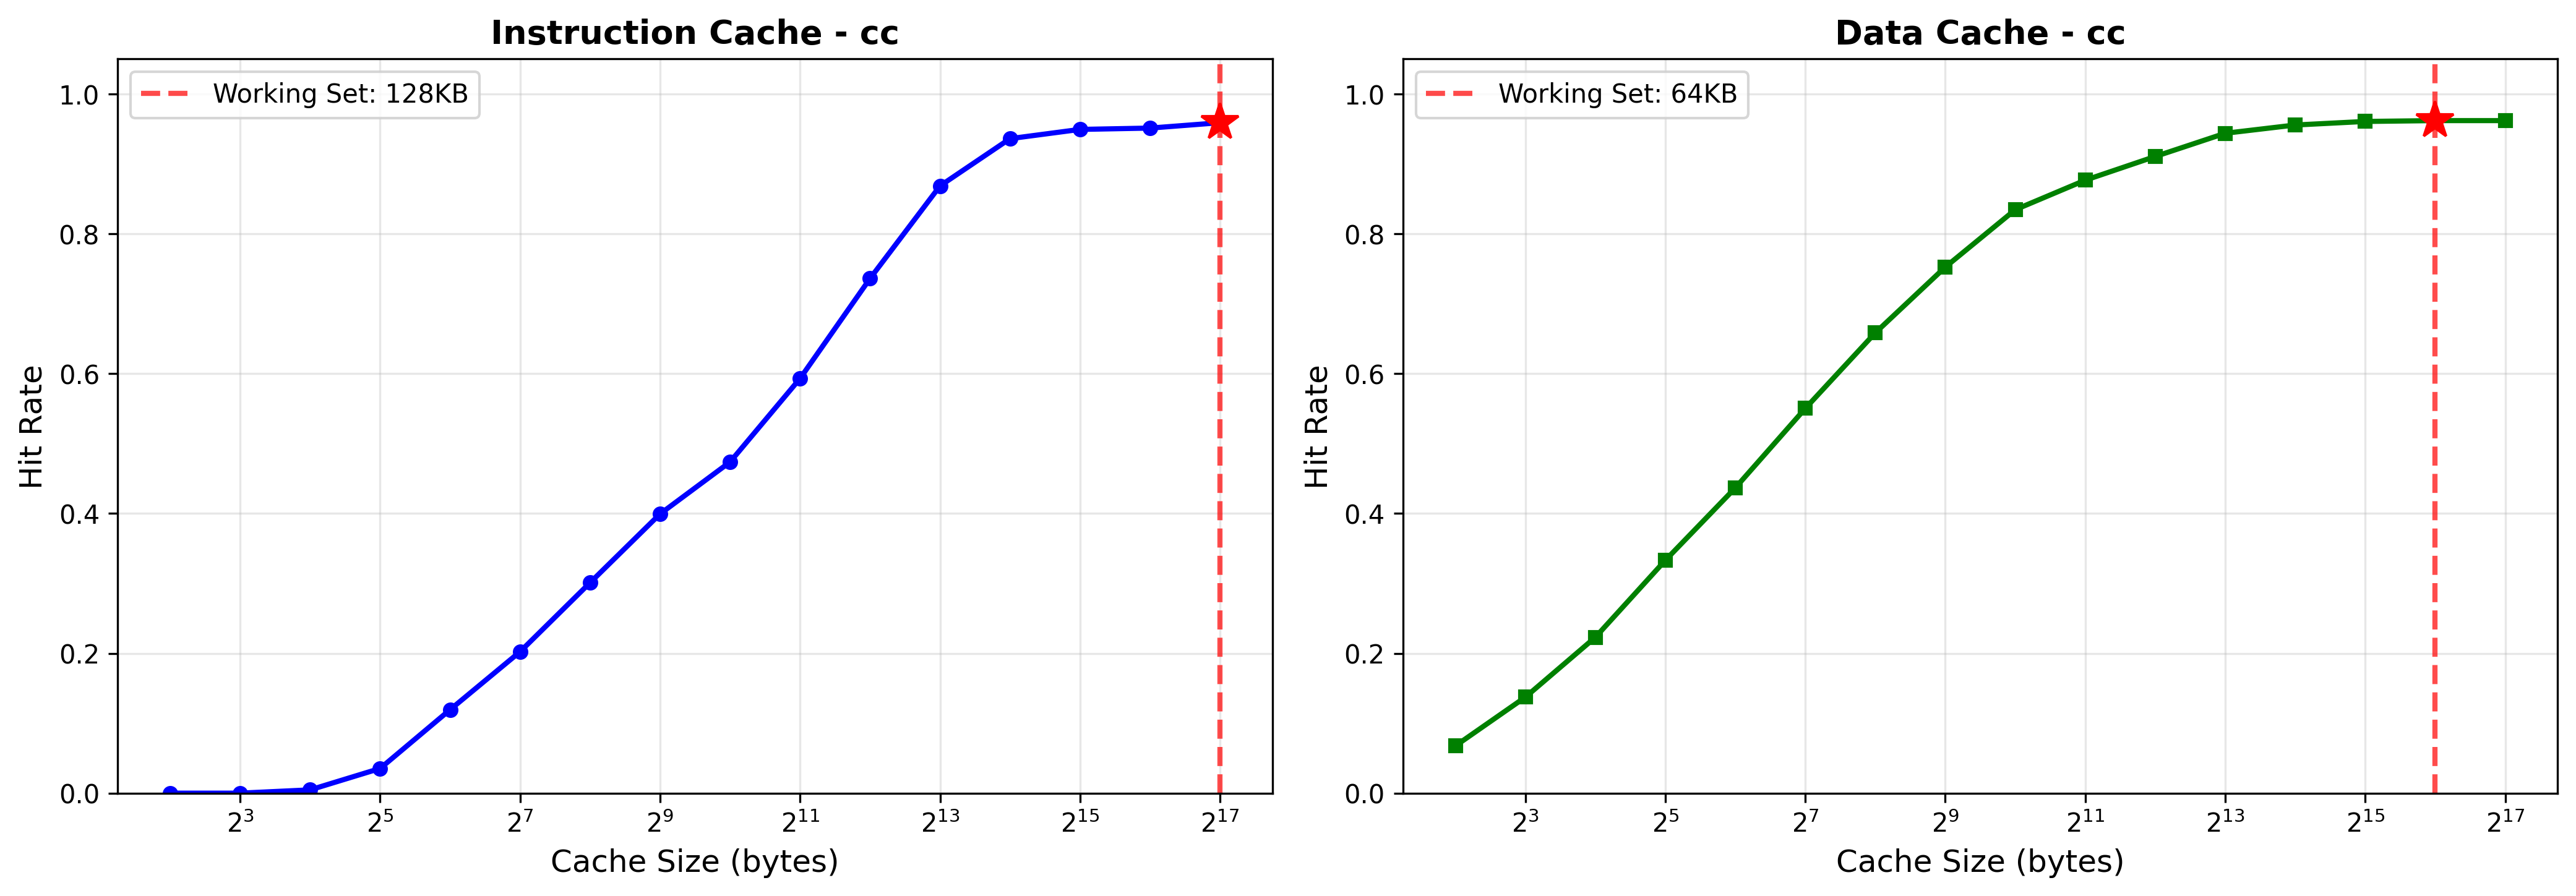
\includegraphics[width=0.8\textwidth]{working_set_cc.png}
\caption{CC trace 工作集特征曲线}
\end{figure}

\begin{figure}[H]
\centering
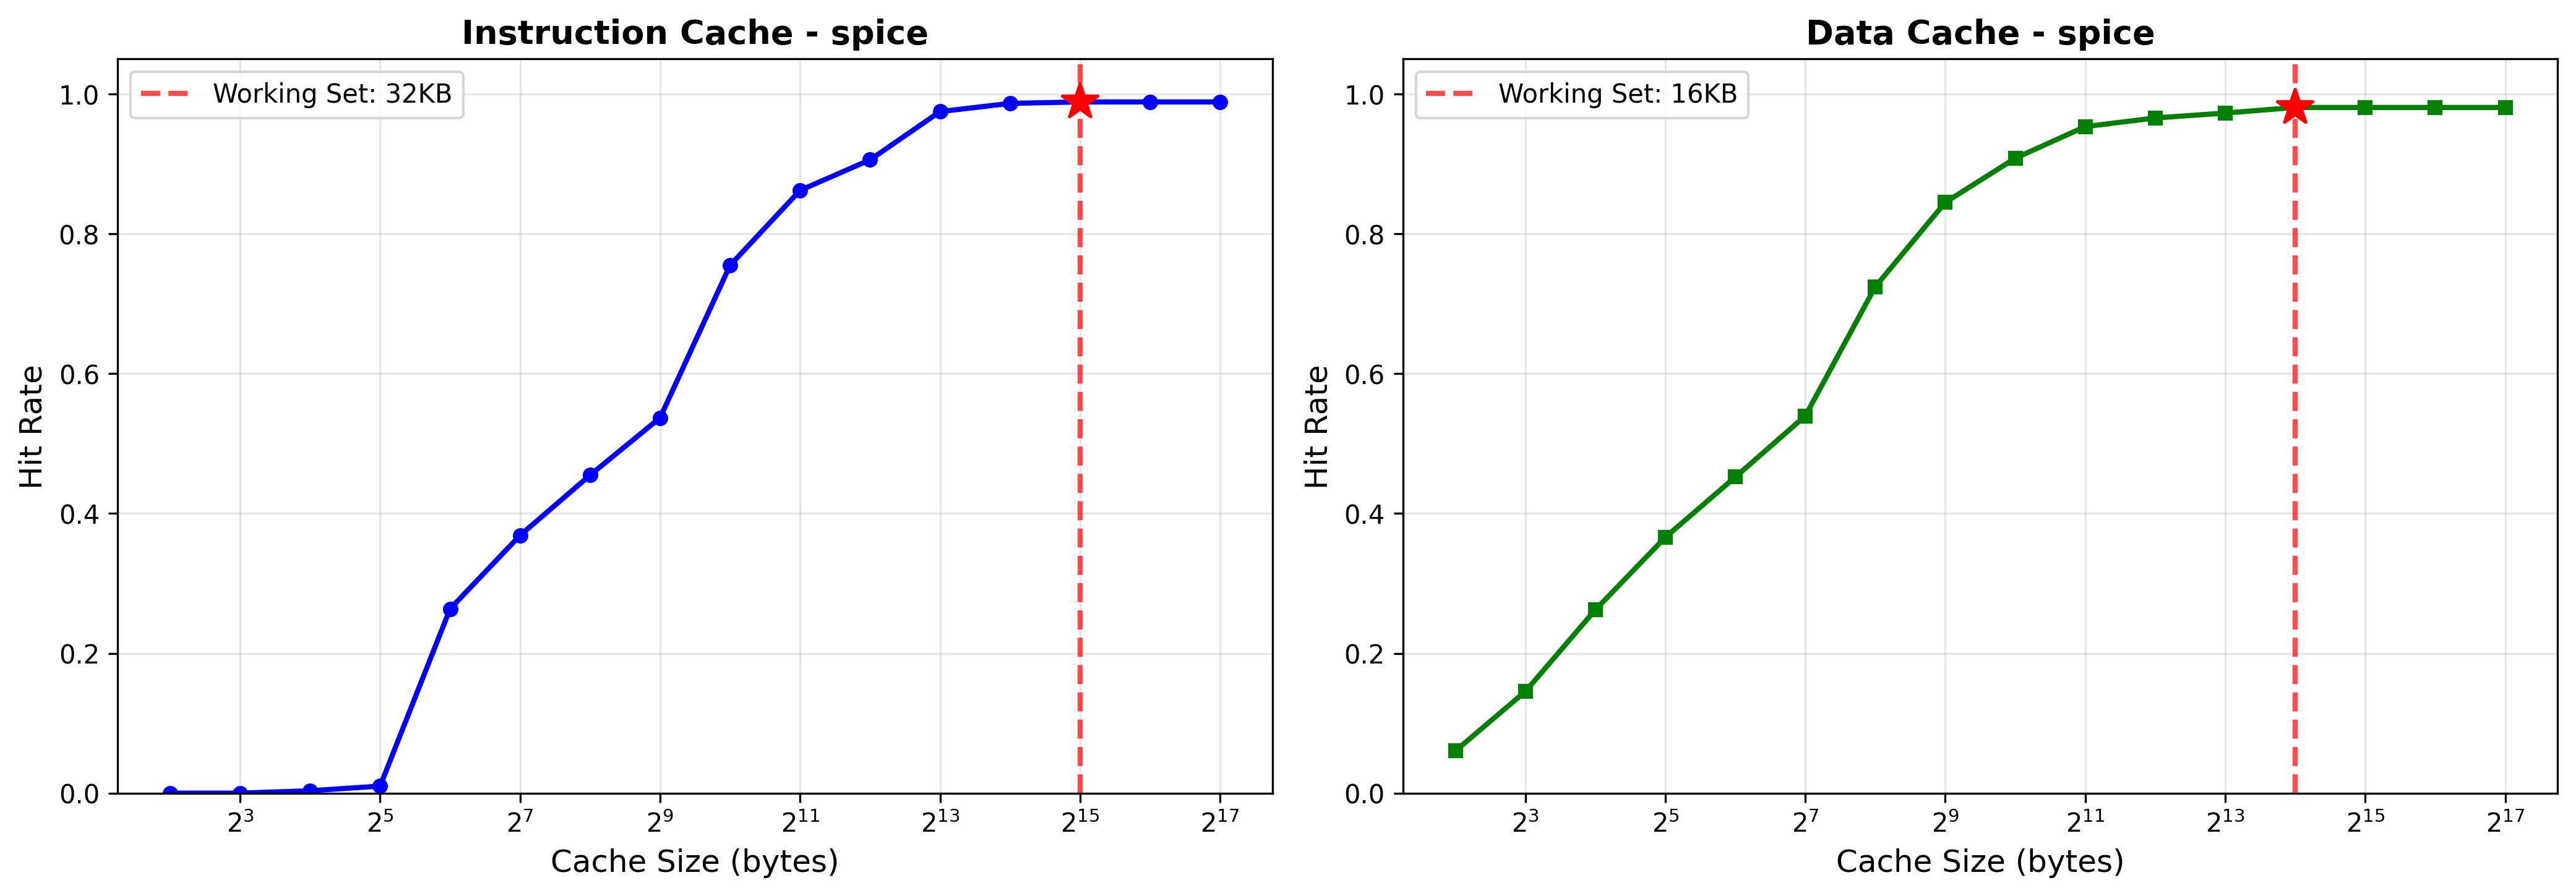
\includegraphics[width=0.8\textwidth]{working_set_spice.png}
\caption{SPICE trace 工作集特征曲线}
\end{figure}

\begin{figure}[H]
\centering
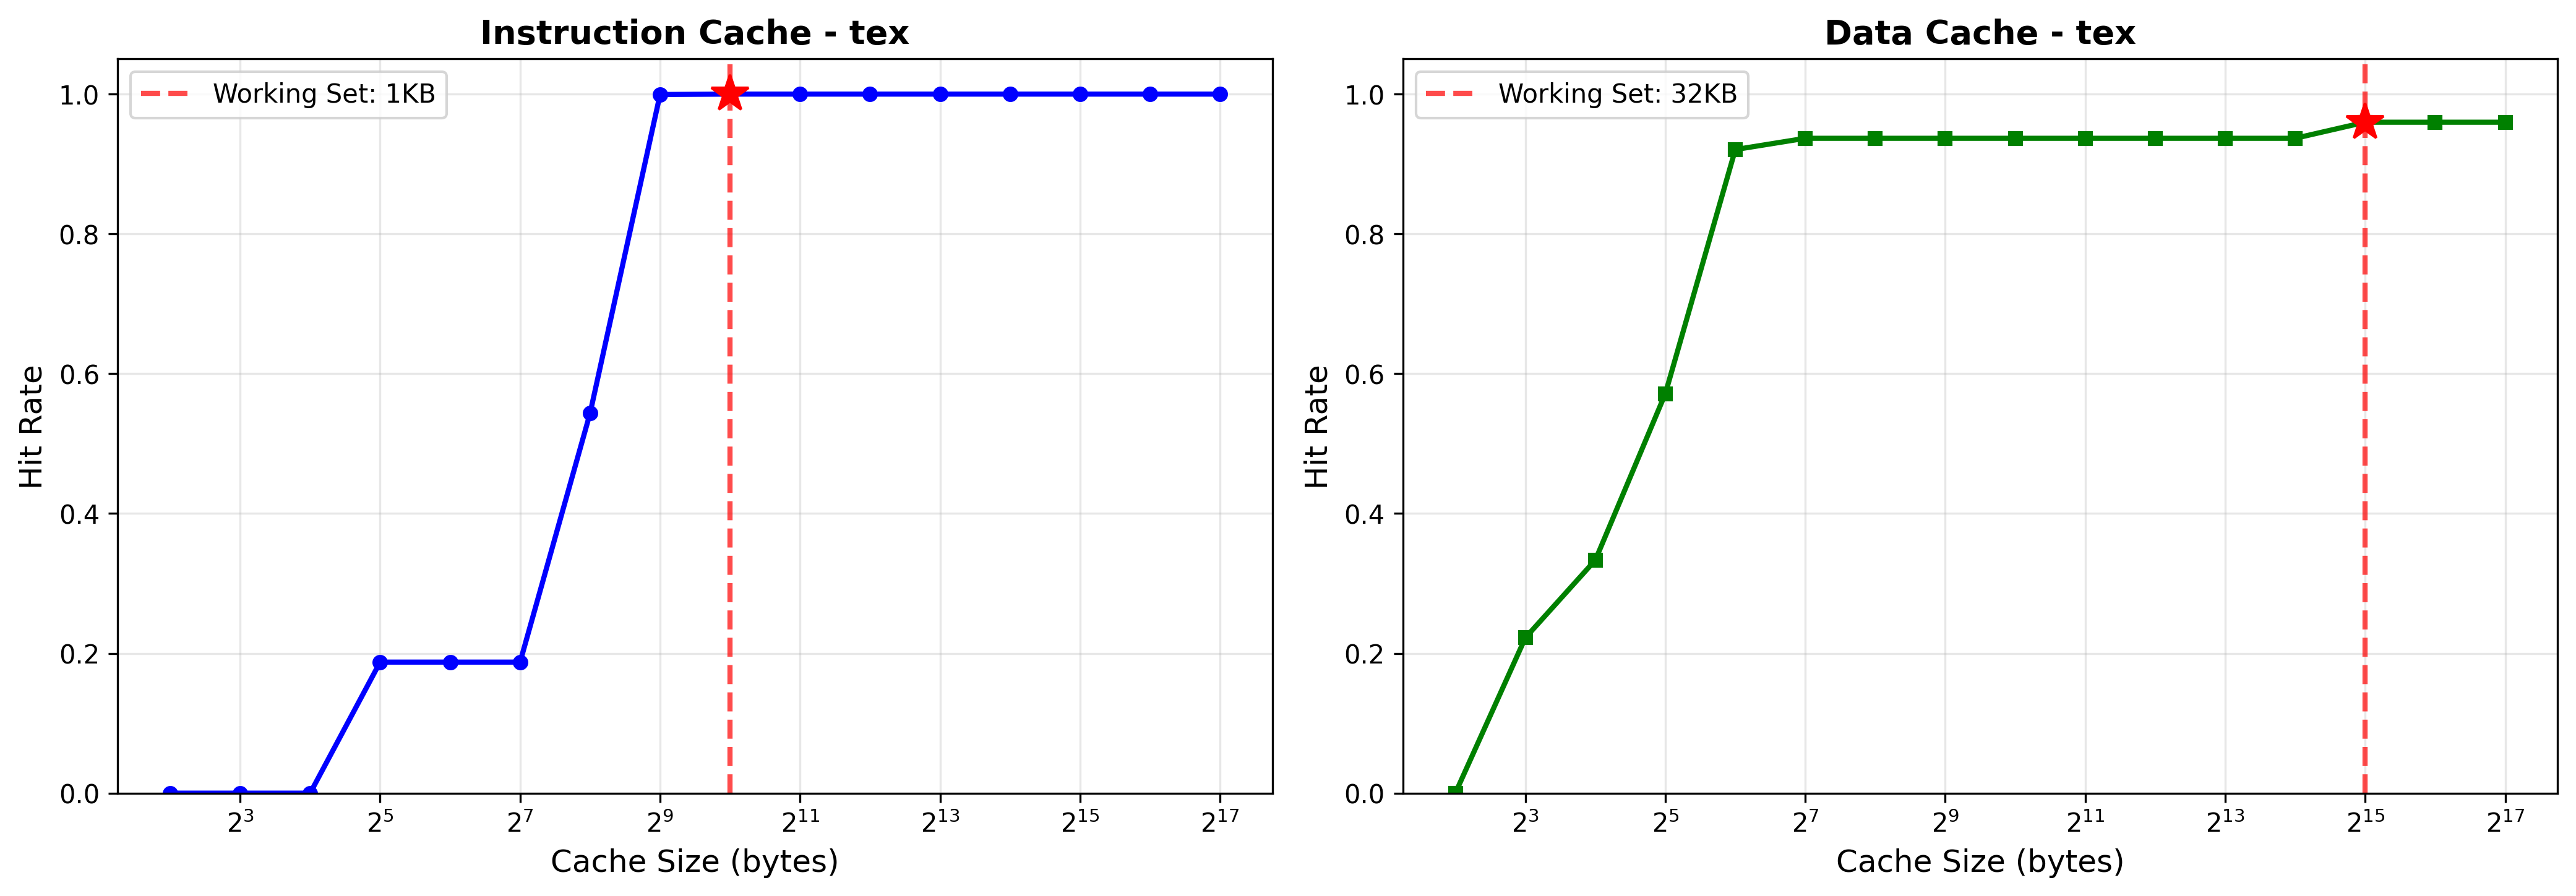
\includegraphics[width=0.8\textwidth]{working_set_tex.png}
\caption{TEX trace 工作集特征曲线}
\end{figure}

\subsubsection{结果分析}

\textbf{工作集大小（命中率饱和时的 Cache 大小）：}

\begin{table}[H]
\centering
\begin{tabular}{|l|c|c|}
\hline
\textbf{Trace} & \textbf{指令工作集} & \textbf{数据工作集} \\
\hline
cc & $>$128 KB & $\approx$64 KB \\
spice & $\approx$32 KB & $\approx$16 KB \\
tex & $\approx$1 KB & $\approx$32 KB \\
\hline
\end{tabular}
\end{table}

\textbf{曲线特征解释：}

\begin{table}[H]
\centering
\small
\begin{tabular}{p{3.5cm}p{5cm}p{6cm}}
\toprule
\textbf{阶段} & \textbf{表现} & \textbf{原因} \\
\midrule
初始陡升段 & 缓存从极小增长时，命中率快速提升 & 容量缺失（Capacity Miss）占主导，增加缓存直接减少缺失 \\
\midrule
拐点（Knee Point） & 命中率增长放缓，标志工作集大小的近似值 & 缓存足以容纳大部分活跃数据/指令 \\
\midrule
平台段 & 命中率趋于稳定，继续增大缓存收益递减 & 剩余缺失主要是强制缺失（Compulsory Miss）和非重复访问容量缺失 \\
\bottomrule
\end{tabular}
\caption{Cache 命中率随大小变化的四个阶段}
\end{table}

\textbf{应用特征分析：}

\begin{table}[H]
\centering
\small
\caption{三个 Trace 的工作集特征分析}
\begin{tabular}{p{2.5cm}p{3cm}p{9cm}}
\toprule
\textbf{Trace 名称} & \textbf{工作集大小} & \textbf{特征解释} \\
\midrule
cc（编译器） & 指令: $>$128 KB\newline 数据: $\approx$64 KB & 指令工作集极大，反映复杂的控制流和多个编译阶段；数据工作集中等，涉及符号表和中间代码 \\
\midrule
spice（电路仿真） & 指令: $\approx$32 KB\newline 数据: $\approx$16 KB & 两者都较小，说明核心计算循环紧凑，数据访问集中 \\
\midrule
tex（文档处理） & 指令: $\approx$1 KB\newline 数据: $\approx$32 KB & 指令工作集极小，表明极紧密的循环；\newline 数据工作集大，处理大量文档数据 \\
\bottomrule
\end{tabular}
\end{table}
\subsection{实验2：块大小的影响 (Impact of Block Size)}

\subsubsection{实验设计}

固定缓存大小和相联度，测试不同块大小对命中率的影响：

\begin{lstlisting}[language=Python]
BLOCK_SIZES = [2**i for i in range(2, 13)]  # 4B到4KB
CACHE_SIZE = 8192       # 每个缓存8KB
ASSOCIATIVITY = 2       # 2路组相联

def run_simulation(trace_path, block_size):
    cmd = [sim_path, "-is", "8192", "-ds", "8192",
           "-bs", str(block_size), "-a", "2",
           "-wb", "-wa", trace_path]
    # 解析I-cache和D-cache命中率...
\end{lstlisting}

每个 trace 运行 22 次模拟（11 个块大小 × 2 种缓存类型）。

\subsubsection{实验结果}

\begin{figure}[H]
\centering
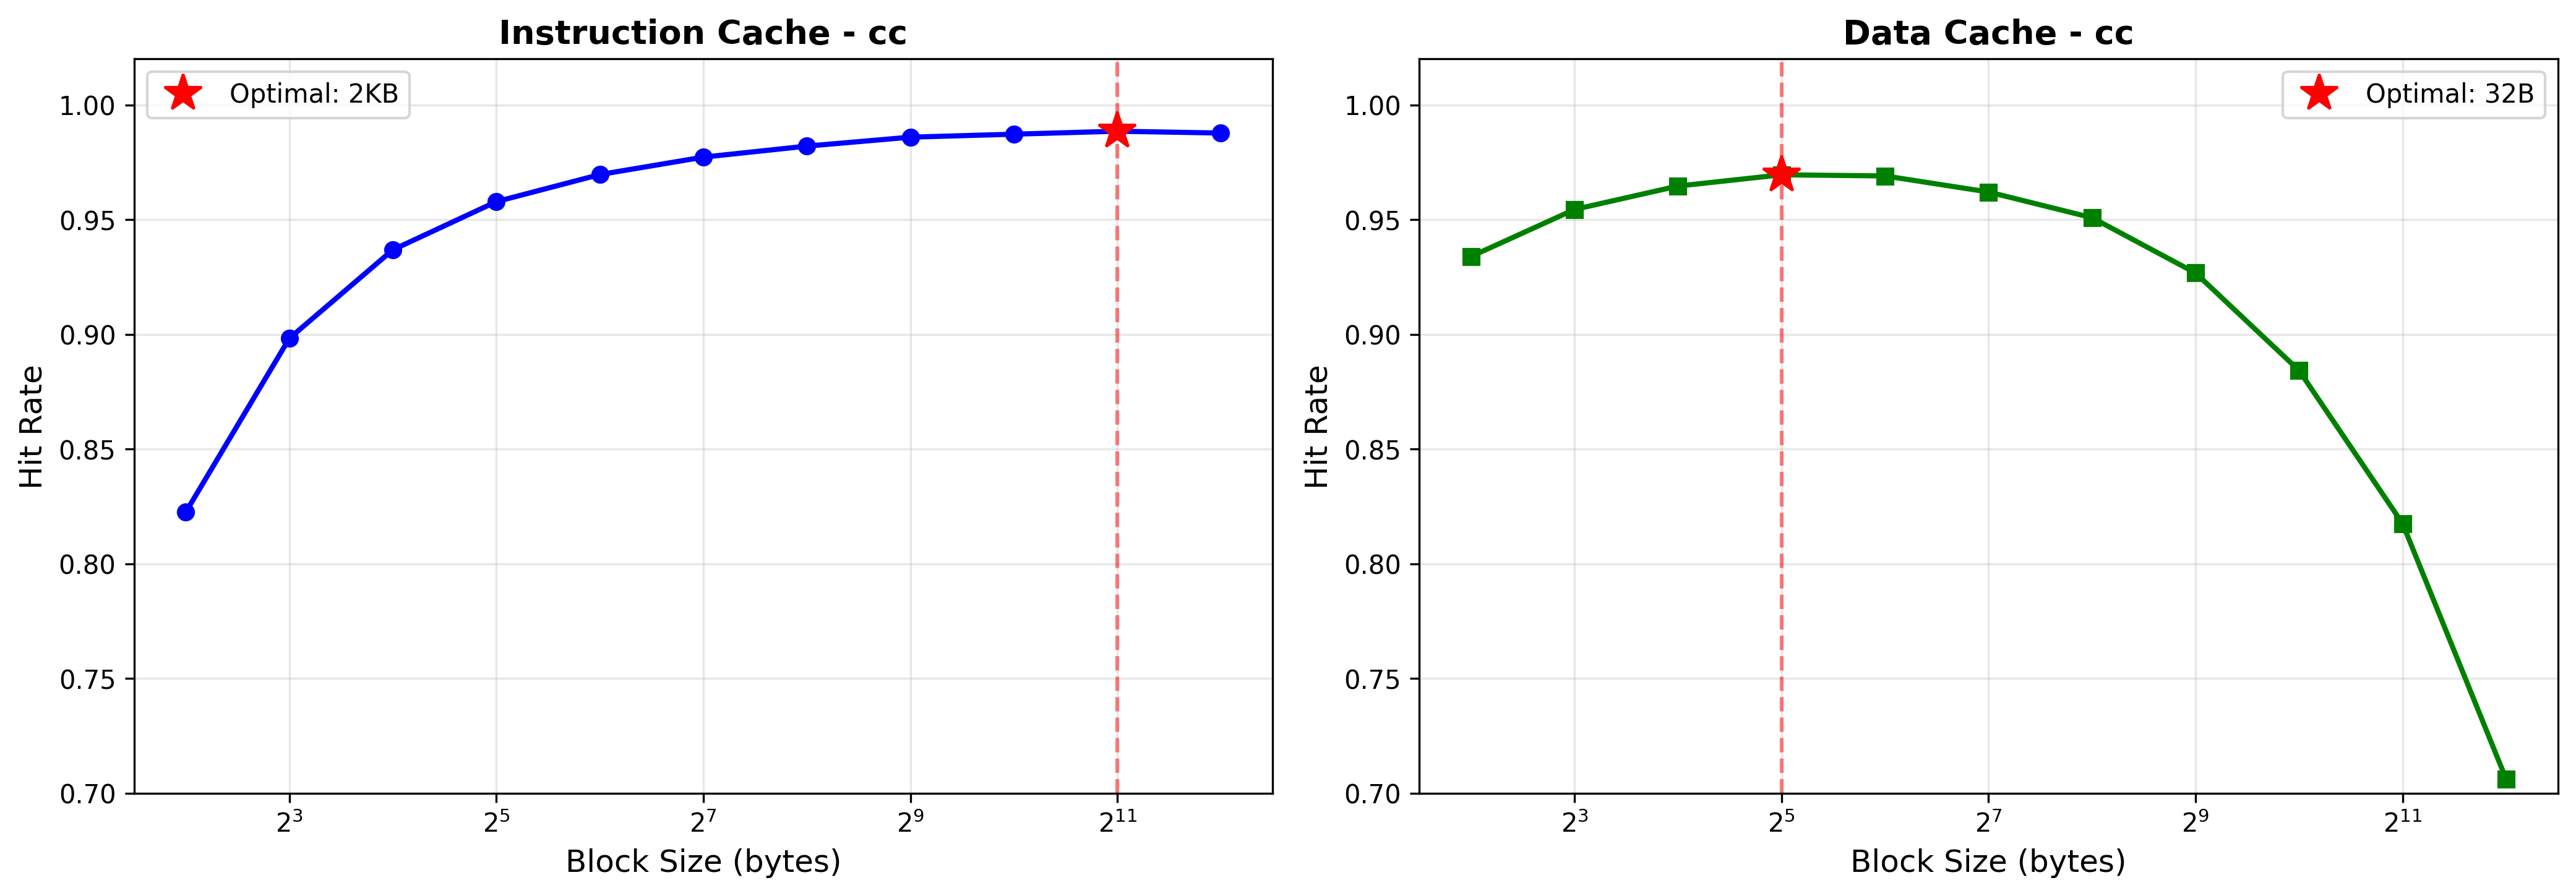
\includegraphics[width=0.8\textwidth]{block_size_impact_cc.png}
\caption{CC trace 块大小影响}
\end{figure}

\begin{figure}[H]
\centering
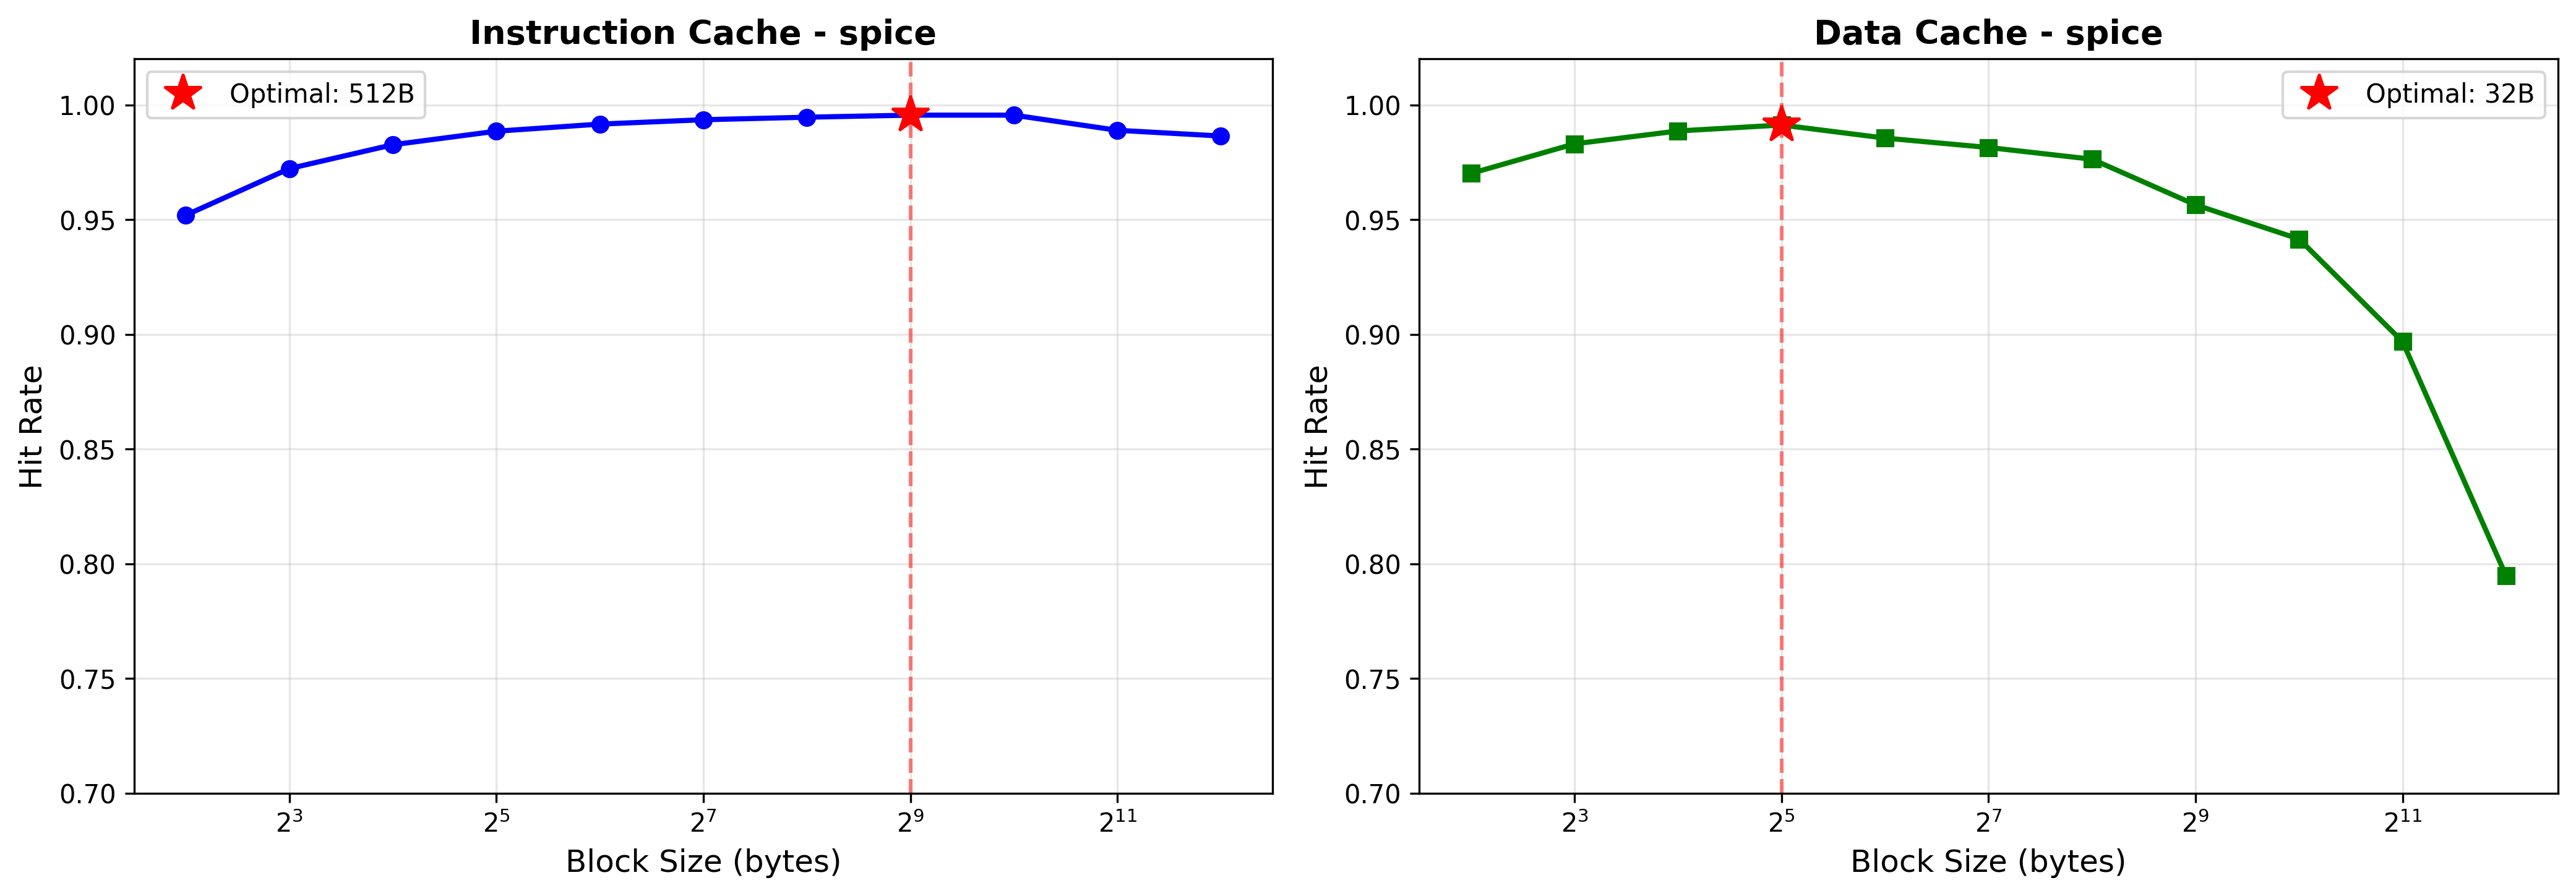
\includegraphics[width=0.8\textwidth]{block_size_impact_spice.png}
\caption{SPICE trace 块大小影响}
\end{figure}

\begin{figure}[H]
\centering
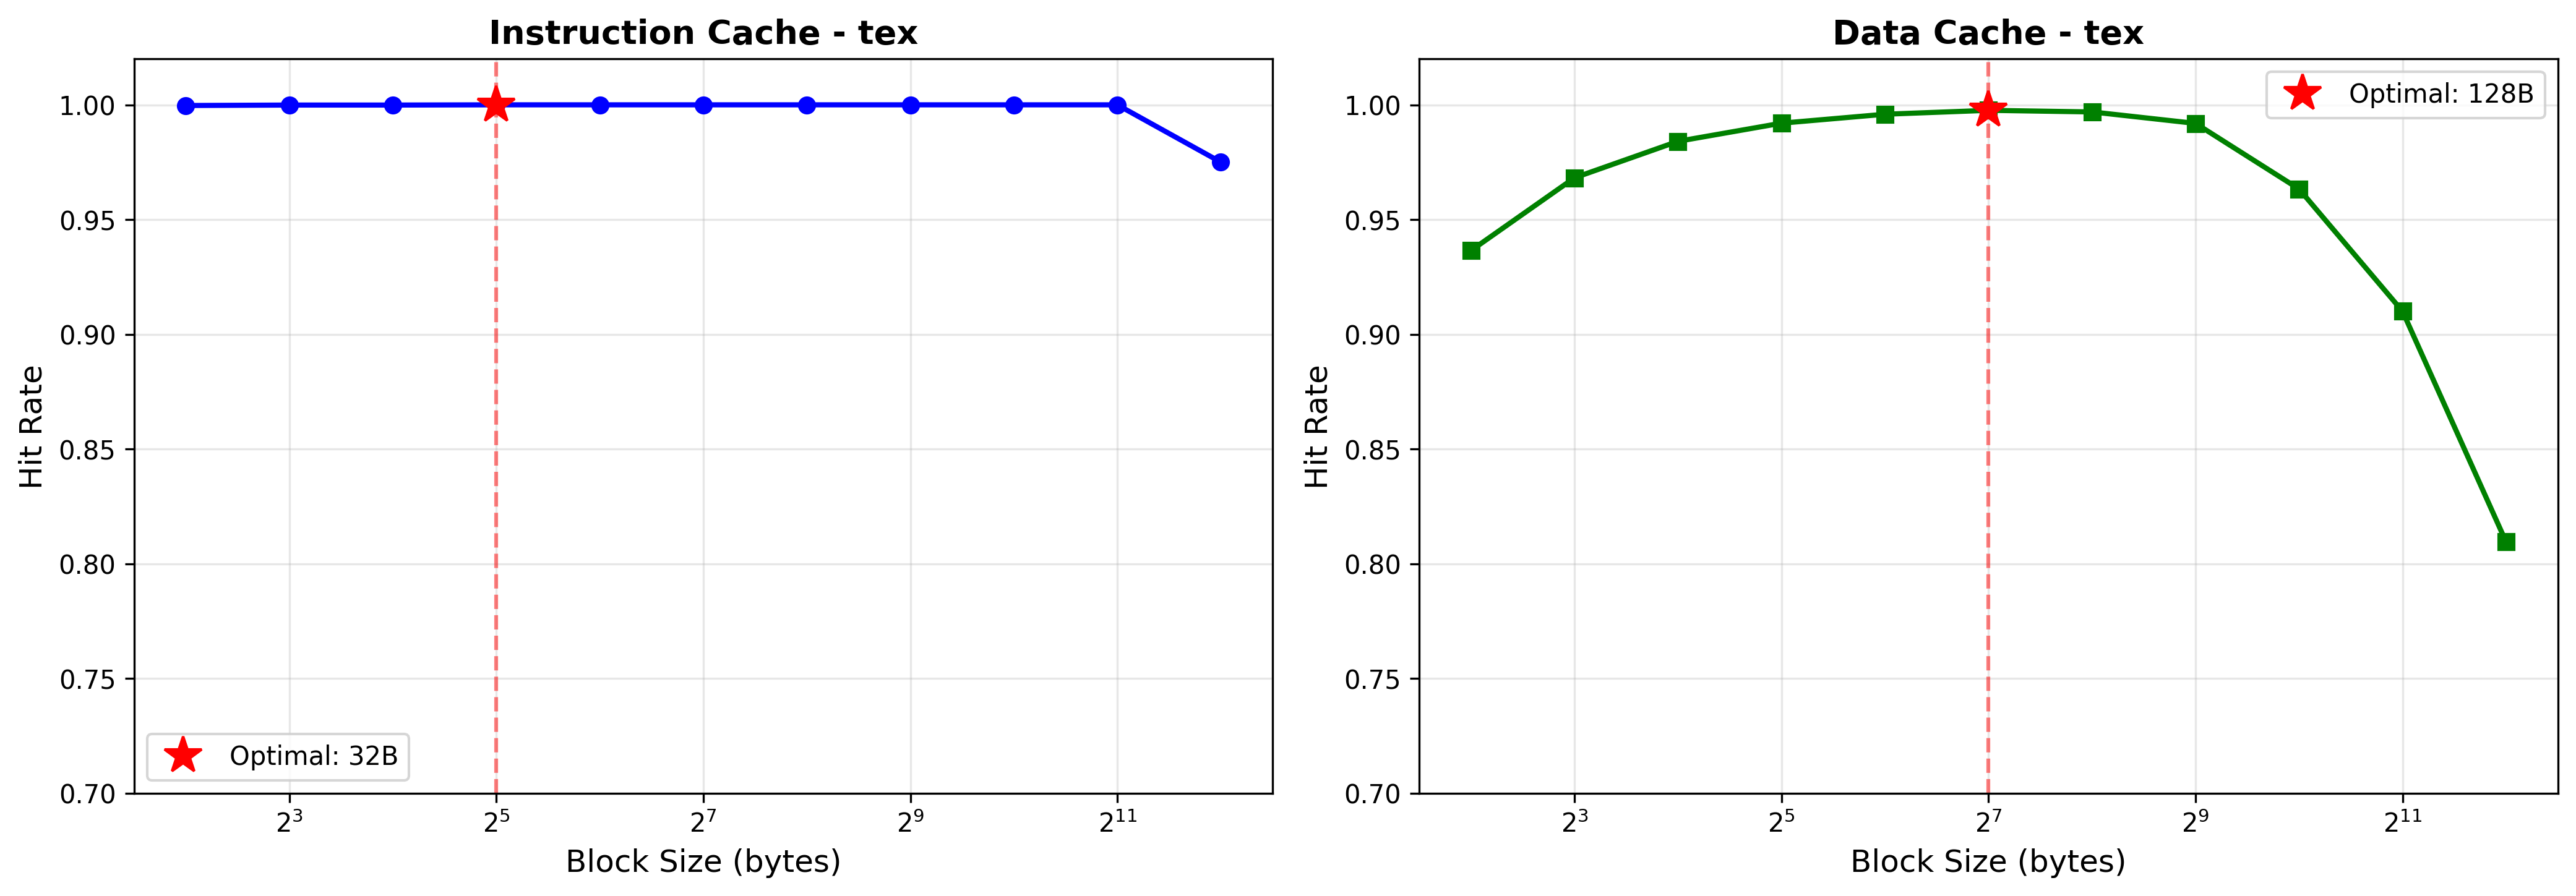
\includegraphics[width=0.8\textwidth]{block_size_impact_tex.png}
\caption{TEX trace 块大小影响}
\end{figure}

\subsubsection{结果分析}

\textbf{最优块大小：}

\begin{table}[H]
\centering
\begin{tabular}{|l|c|c|}
\hline
\textbf{Trace} & \textbf{I-Cache 最优} & \textbf{D-Cache 最优} \\
\hline
cc & 2048 B (98.85\%) & 32 B (96.95\%) \\
spice & 512 B (99.55\%) & 32 B (99.12\%) \\
tex & 32 B (100.00\%) & 128 B (99.76\%) \\
\hline
\end{tabular}
\end{table}

\textbf{曲线形状解释：}

\begin{table}[H]
\centering
\small
\caption{块大小对命中率影响的曲线形状解释}
\begin{tabular}{p{3.5cm}p{11cm}}
\toprule
\textbf{曲线阶段} & \textbf{原因解释} \\
\midrule
初始上升（小块大小） & 块增大利用了\textbf{空间局部性（Spatial Locality）}。当程序访问地址 $X$ 后，很可能访问 $X+1, X+2$ 等邻近地址。较大的块预取这些数据，减少后续缺失 \\
\midrule
峰值/平台（最优块大小） & 达到空间局部性利用和缓存污染的最佳平衡点 \\
\midrule
下降（大块大小） & \textbf{缓存污染}：过大的块带入许多不会被使用的字节，浪费缓存空间\newline
\textbf{缓存行减少}：固定 8KB，块为 4KB 时只有 2 行，灵活性大幅下降，冲突缺失增加\newline
\textbf{空间局部性有限}：若程序访问模式跳跃性强，大块的额外数据无用武之地 \\
\bottomrule
\end{tabular}
\end{table}

\textbf{指令与数据的差异：}

\textbf{指令最优块通常大于数据最优块。}这是因为指令执行具有强顺序性，程序计数器顺序递增，循环体重复执行相同指令序列，能充分利用大块带来的空间局部性；而数据访问模式取决于具体的数据结构，链表、树等指针结构的跳跃访问使得过大的块会带入无用数据，造成缓存污染。

\begin{itemize}
    \item \textbf{指令引用}：通常具有\textbf{强顺序空间局部性}。程序顺序执行指令，循环和顺序代码块受益于大块。cc 和 spice 的 I-cache 最优块达到 512B-2KB。
    
    \item \textbf{数据引用}：访问模式取决于数据结构。数组遍历有高空间局部性，链表/指针结构则局部性差。大多数情况下 D-cache 最优块较小（32B-128B）。
    
    \item \textbf{tex 的特殊性}：I-cache 最优仅 32B，说明代码路径高度分支化；D-cache 为 128B，表明处理连续的文档数据。
\end{itemize}
\subsection{实验3：关联度的影响 (Impact of Associativity)}

\subsubsection{实验设计}

固定缓存大小和块大小，测试相联度对命中率的影响：

\begin{lstlisting}[language=Python]
ASSOCIATIVITIES = [2**i for i in range(0, 7)]  # 1到64
CACHE_SIZE = 8192       # 8 KB
BLOCK_SIZE = 128        # 128 bytes

def run_simulation(trace_path, associativity):
    cmd = [sim_path, "-is", "8192", "-ds", "8192",
           "-bs", "128", "-a", str(associativity),
           "-wb", "-wa", trace_path]
\end{lstlisting}

每个 trace 测试 14 次（7 个相联度 × 2 种缓存）。

\subsubsection{实验结果}

\begin{figure}[H]
\centering
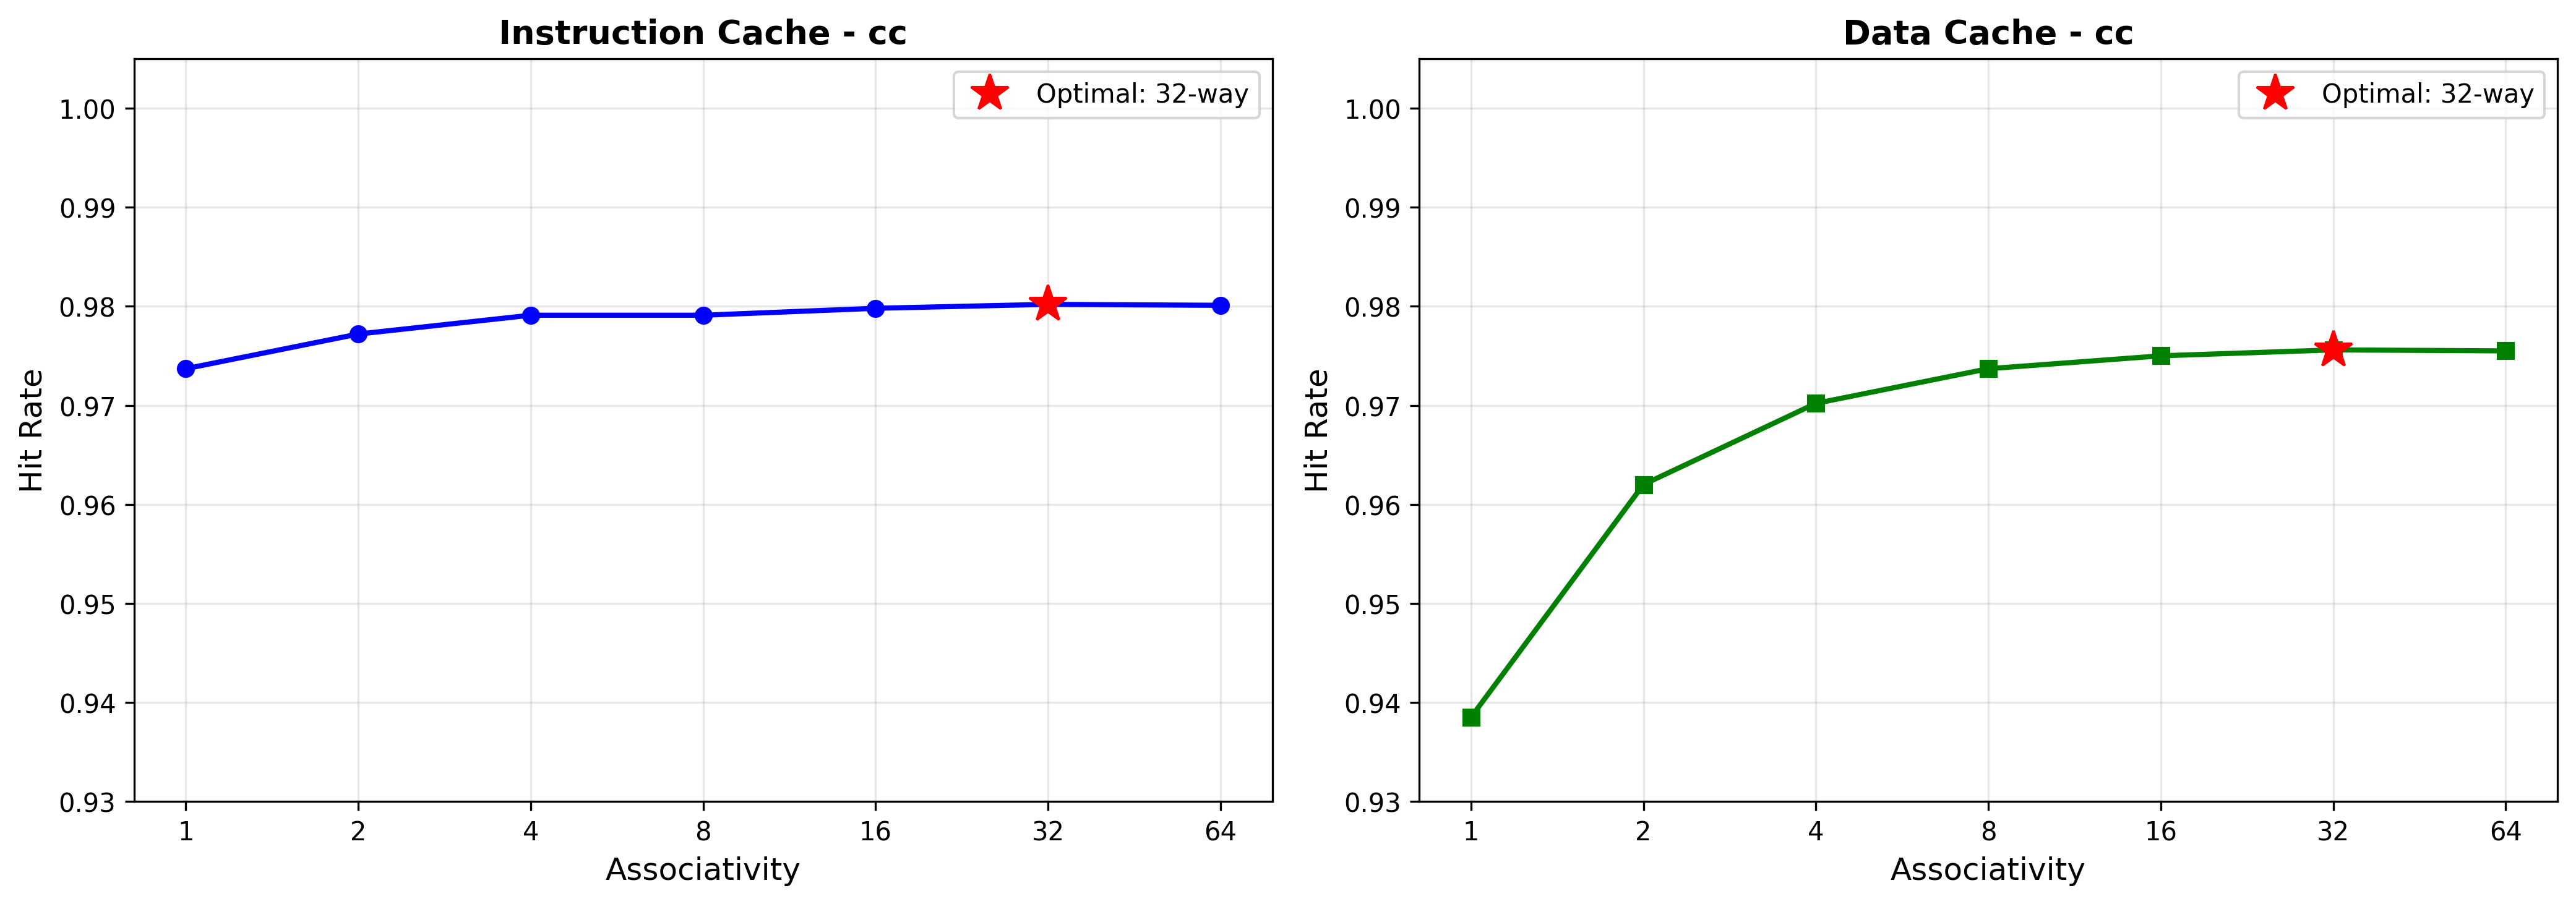
\includegraphics[width=0.8\textwidth]{associativity_cc.png}
\caption{CC trace 相联度影响}
\end{figure}

\begin{figure}[H]
\centering
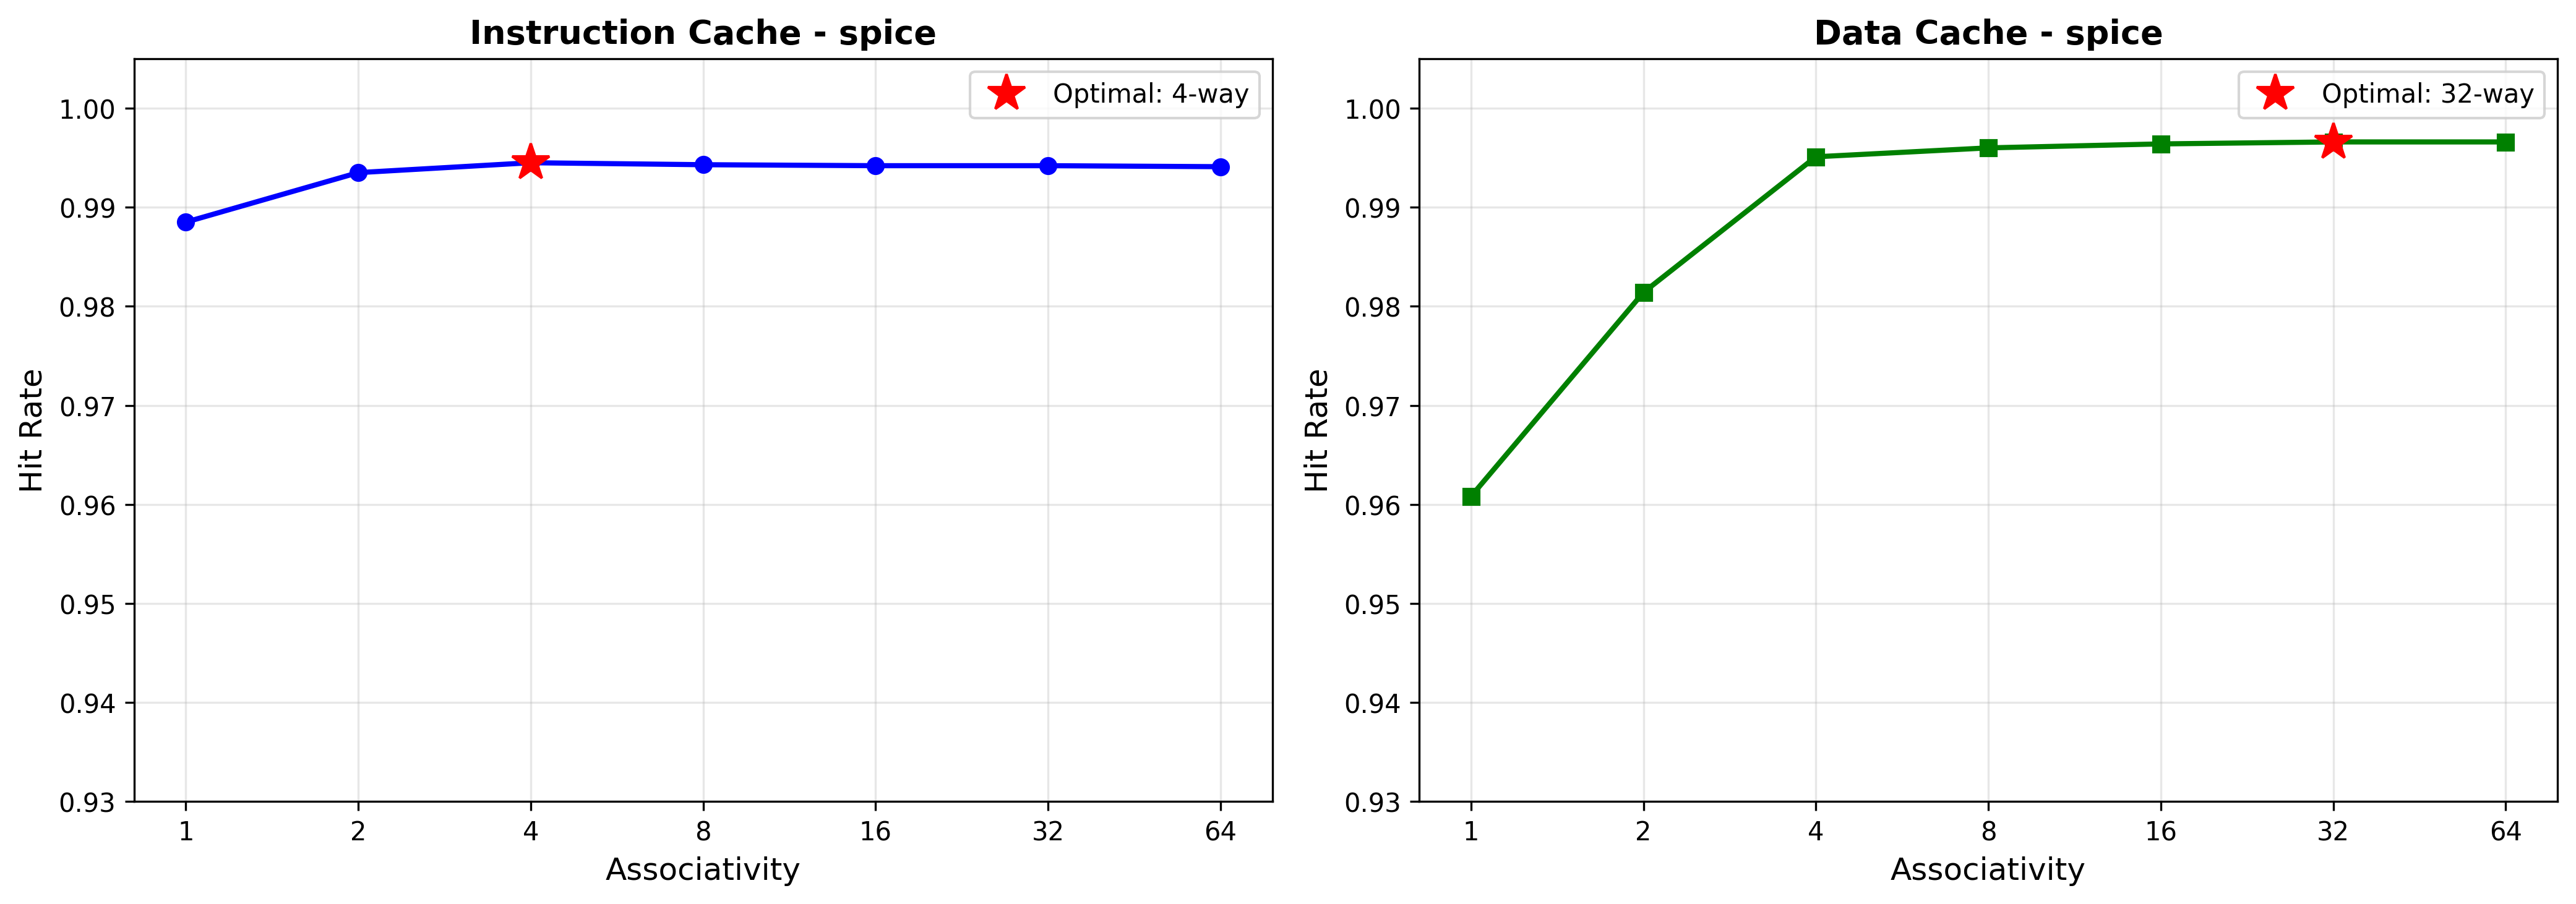
\includegraphics[width=0.8\textwidth]{associativity_spice.png}
\caption{SPICE trace 相联度影响}
\end{figure}

\begin{figure}[H]
\centering
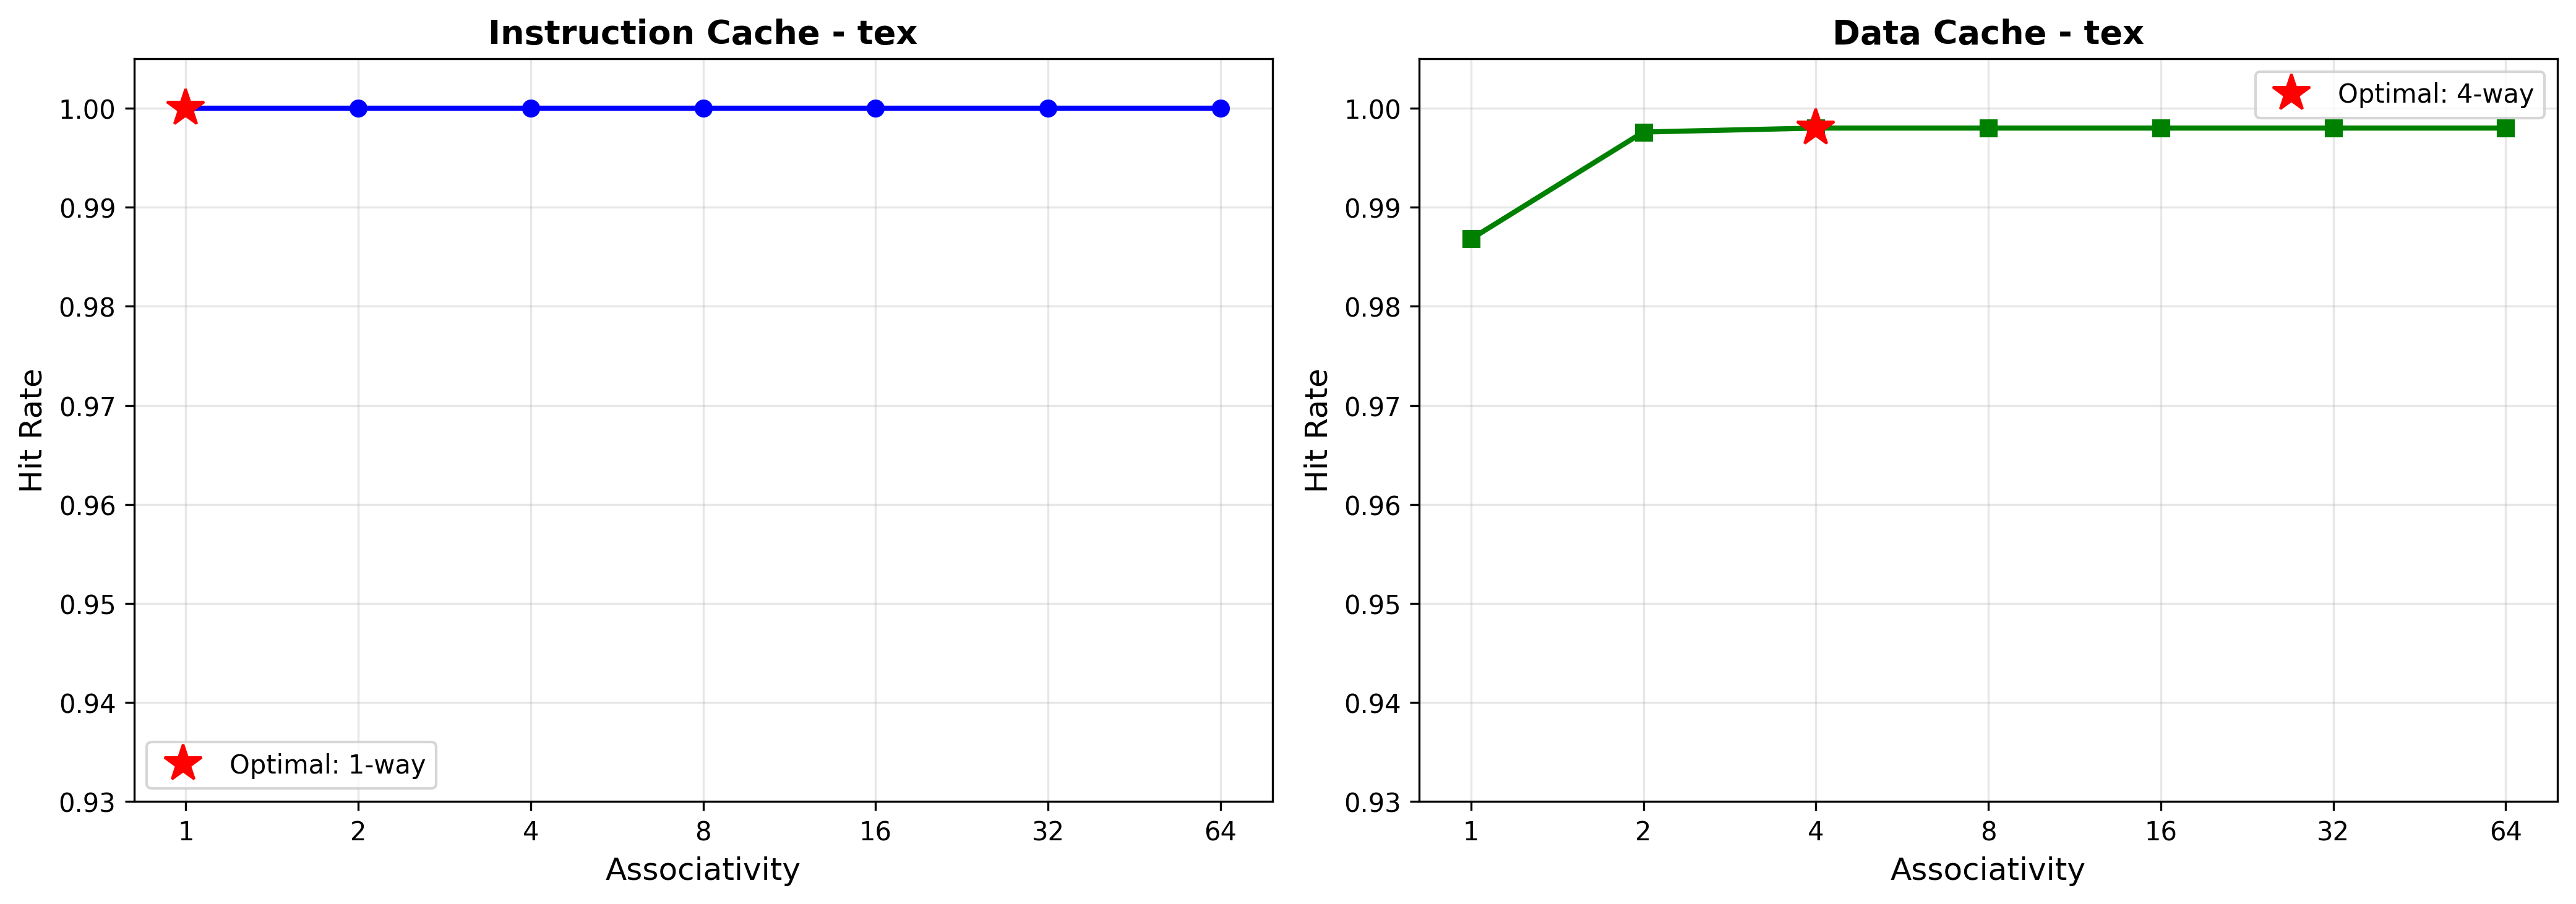
\includegraphics[width=0.8\textwidth]{associativity_tex.png}
\caption{TEX trace 相联度影响}
\end{figure}

\subsubsection{结果分析}

\textbf{最优相联度：}

\begin{table}[H]
\centering
\begin{tabular}{|l|c|c|}
\hline
\textbf{Trace} & \textbf{I-Cache} & \textbf{D-Cache} \\
\hline
cc & 32-way (98.02\%) & 32-way (97.56\%) \\
spice & 4-way (99.45\%) & 32-way (99.66\%) \\
tex & 1-way (100.00\%) & 4-way (99.80\%) \\
\hline
\end{tabular}
\end{table}

\textbf{注：此处最优相联度指命中率最高（或无法区分）时最小的相联度。}

\textbf{曲线形状解释：}

\begin{table}[H]
\centering
\small
\caption{相联度对命中率影响的曲线形状解释}
\begin{tabular}{p{4cm}p{11cm}}
\toprule
\textbf{曲线阶段} & \textbf{原因解释} \\
\midrule
初始陡升（低相联度） & 直接映射缓存（1-way）遭受大量\textbf{冲突缺失（Conflict Miss）}。多个内存块映射到同一 Set 时互相驱逐。从 1-way 到 2-way、4-way 的改进最显著 \\
\midrule
收益递减（中等相联度） & 8-way、16-way 时大部分冲突已消除，曲线趋平 \\
\midrule
平台（高相联度） & 32-way、64-way 时命中率不再提升。剩余缺失是容量缺失和强制缺失，无法通过相联度解决 \\
\midrule
递减律 & 相联度翻倍的收益逐步下降。$1\to2$ 改进远大于 $32\to64$ \\
\bottomrule
\end{tabular}
\end{table}

\textbf{指令与数据的差异：}

\textbf{数据引用对相联度更敏感，指令引用对相联度较不敏感。}指令访问由程序计数器驱动，具有高度的顺序性和规律性，即使在直接映射（1-way）缓存中也很少发生地址冲突；而数据访问涉及多种数据结构（符号表、临时变量、堆栈等），地址分布更加分散，容易映射到相同的缓存组造成冲突缺失，因此需要更高的相联度来缓解。

\begin{table}[H]
\centering
\small
\caption{指令与数据缓存对相联度的敏感性对比}
\begin{tabular}{p{2.5cm}p{6cm}p{6cm}}
\toprule
\textbf{Trace} & \textbf{I-Cache 特征} & \textbf{D-Cache 特征} \\
\midrule
cc & 1-way 到 64-way 改进仅 0.6\%，说明指令访问高度\textbf{顺序化}，冲突缺失极少 & 1-way 到 64-way 改进达 3.7\%，说明数据访问模式\textbf{更分散}，创造更多地址冲突 \\
\midrule
spice & 4-way 即达到最优，指令流较为\textbf{规律} & 需要 32-way 才能达到最优，数据访问存在较多\textbf{随机性} \\
\midrule
tex & 1-way 即达到 100\% 命中率！指令访问\textbf{极度规律}，完全无冲突 & 4-way 即饱和，数据访问也相对规律（文档顺序处理） \\
\bottomrule
\end{tabular}
\end{table}

\clearpage
\textbf{差异原因分析：}

\begin{table}[H]
\centering
\small
\caption{指令引用与数据引用的本质区别}
\begin{tabular}{p{3.5cm}p{5.5cm}p{5.5cm}}
\toprule
\textbf{特征维度} & \textbf{指令引用 (I-Cache)} & \textbf{数据引用 (D-Cache)} \\
\midrule
访问模式 & \textbf{高度顺序化}：程序计数器（PC）顺序递增，循环体重复执行相同指令序列 & \textbf{取决于数据结构}：数组顺序访问，链表/树随机跳转，哈希表散列分布 \\
\midrule
地址分布 & 集中在\textbf{少数代码段}，热点代码（循环、函数）反复执行 & 分散在\textbf{整个数据空间}，符号表、临时变量、堆栈等分布广泛 \\
\midrule
冲突概率 & \textbf{低}：顺序访问自然避免映射到同一 Set & \textbf{高}：不同数据结构的地址可能哈希冲突到同一 Set \\
\midrule
对相联度的需求 & \textbf{较低}：即使 1-way 也能很好工作（如 tex） & \textbf{较高}：需要更多路来容纳冲突的数据块 \\
\bottomrule
\end{tabular}
\end{table}

\textbf{设计启示：}

\begin{itemize}
    \item \textbf{I-cache 设计}：可采用较低相联度（2-4 way），利用指令的强时间/空间局部性，节省硬件成本
    \item \textbf{D-cache 设计}：需要根据应用类型权衡：
    \begin{itemize}
        \item 规律访问（科学计算）：低相联度即可
        \item 随机访问（数据库、编译器）：需要更高相联度或增大缓存容量
    \end{itemize}
    \item \textbf{不对称设计}：现代处理器常采用 I/D 不同相联度的设计（如 I-cache 4-way，D-cache 8-way），这一实验结果验证了该设计的合理性
\end{itemize}

\clearpage
\subsection{实验4：内存带宽 (Memory Bandwidth)}

\subsubsection{实验设计}

本实验分为两部分，比较不同写策略对内存流量的影响：

\begin{lstlisting}[language=Python]
# 实验1：WT vs WB（固定NWA）
EXPERIMENT_1_CONFIGS = [
    {"size": 8192, "block": 64, "assoc": 2},
    {"size": 8192, "block": 128, "assoc": 2},
    {"size": 16384, "block": 64, "assoc": 2},
    {"size": 16384, "block": 128, "assoc": 4},
]

def run_experiment_1(trace_path):
    for config in EXPERIMENT_1_CONFIGS:
        # 运行WT+NWA
        wt_traffic = run_sim(trace, config, "wt", "nw")
        # 运行WB+NWA
        wb_traffic = run_sim(trace, config, "wb", "nw")
        # 计算流量减少比例...

# 实验2：WA vs NWA（固定WB）
def run_experiment_2(trace_path):
    for config in EXPERIMENT_2_CONFIGS:
        wa_traffic = run_sim(trace, config, "wb", "wa")
        nwa_traffic = run_sim(trace, config, "wb", "nw")
\end{lstlisting}

每个实验运行 12 次模拟（4 配置 × 3 trace），测量总内存流量。

\subsubsection{实验结果}

如下图所示：

左图：比较Write-Through和Write-Back在不同配置下产生的总内存流量大小。

右图：展示Write-Through和Write-Back的总流量分别由多少读流量（Demand Fetch）和写流量（Copy Back）组成。
\begin{figure}[H]
\centering
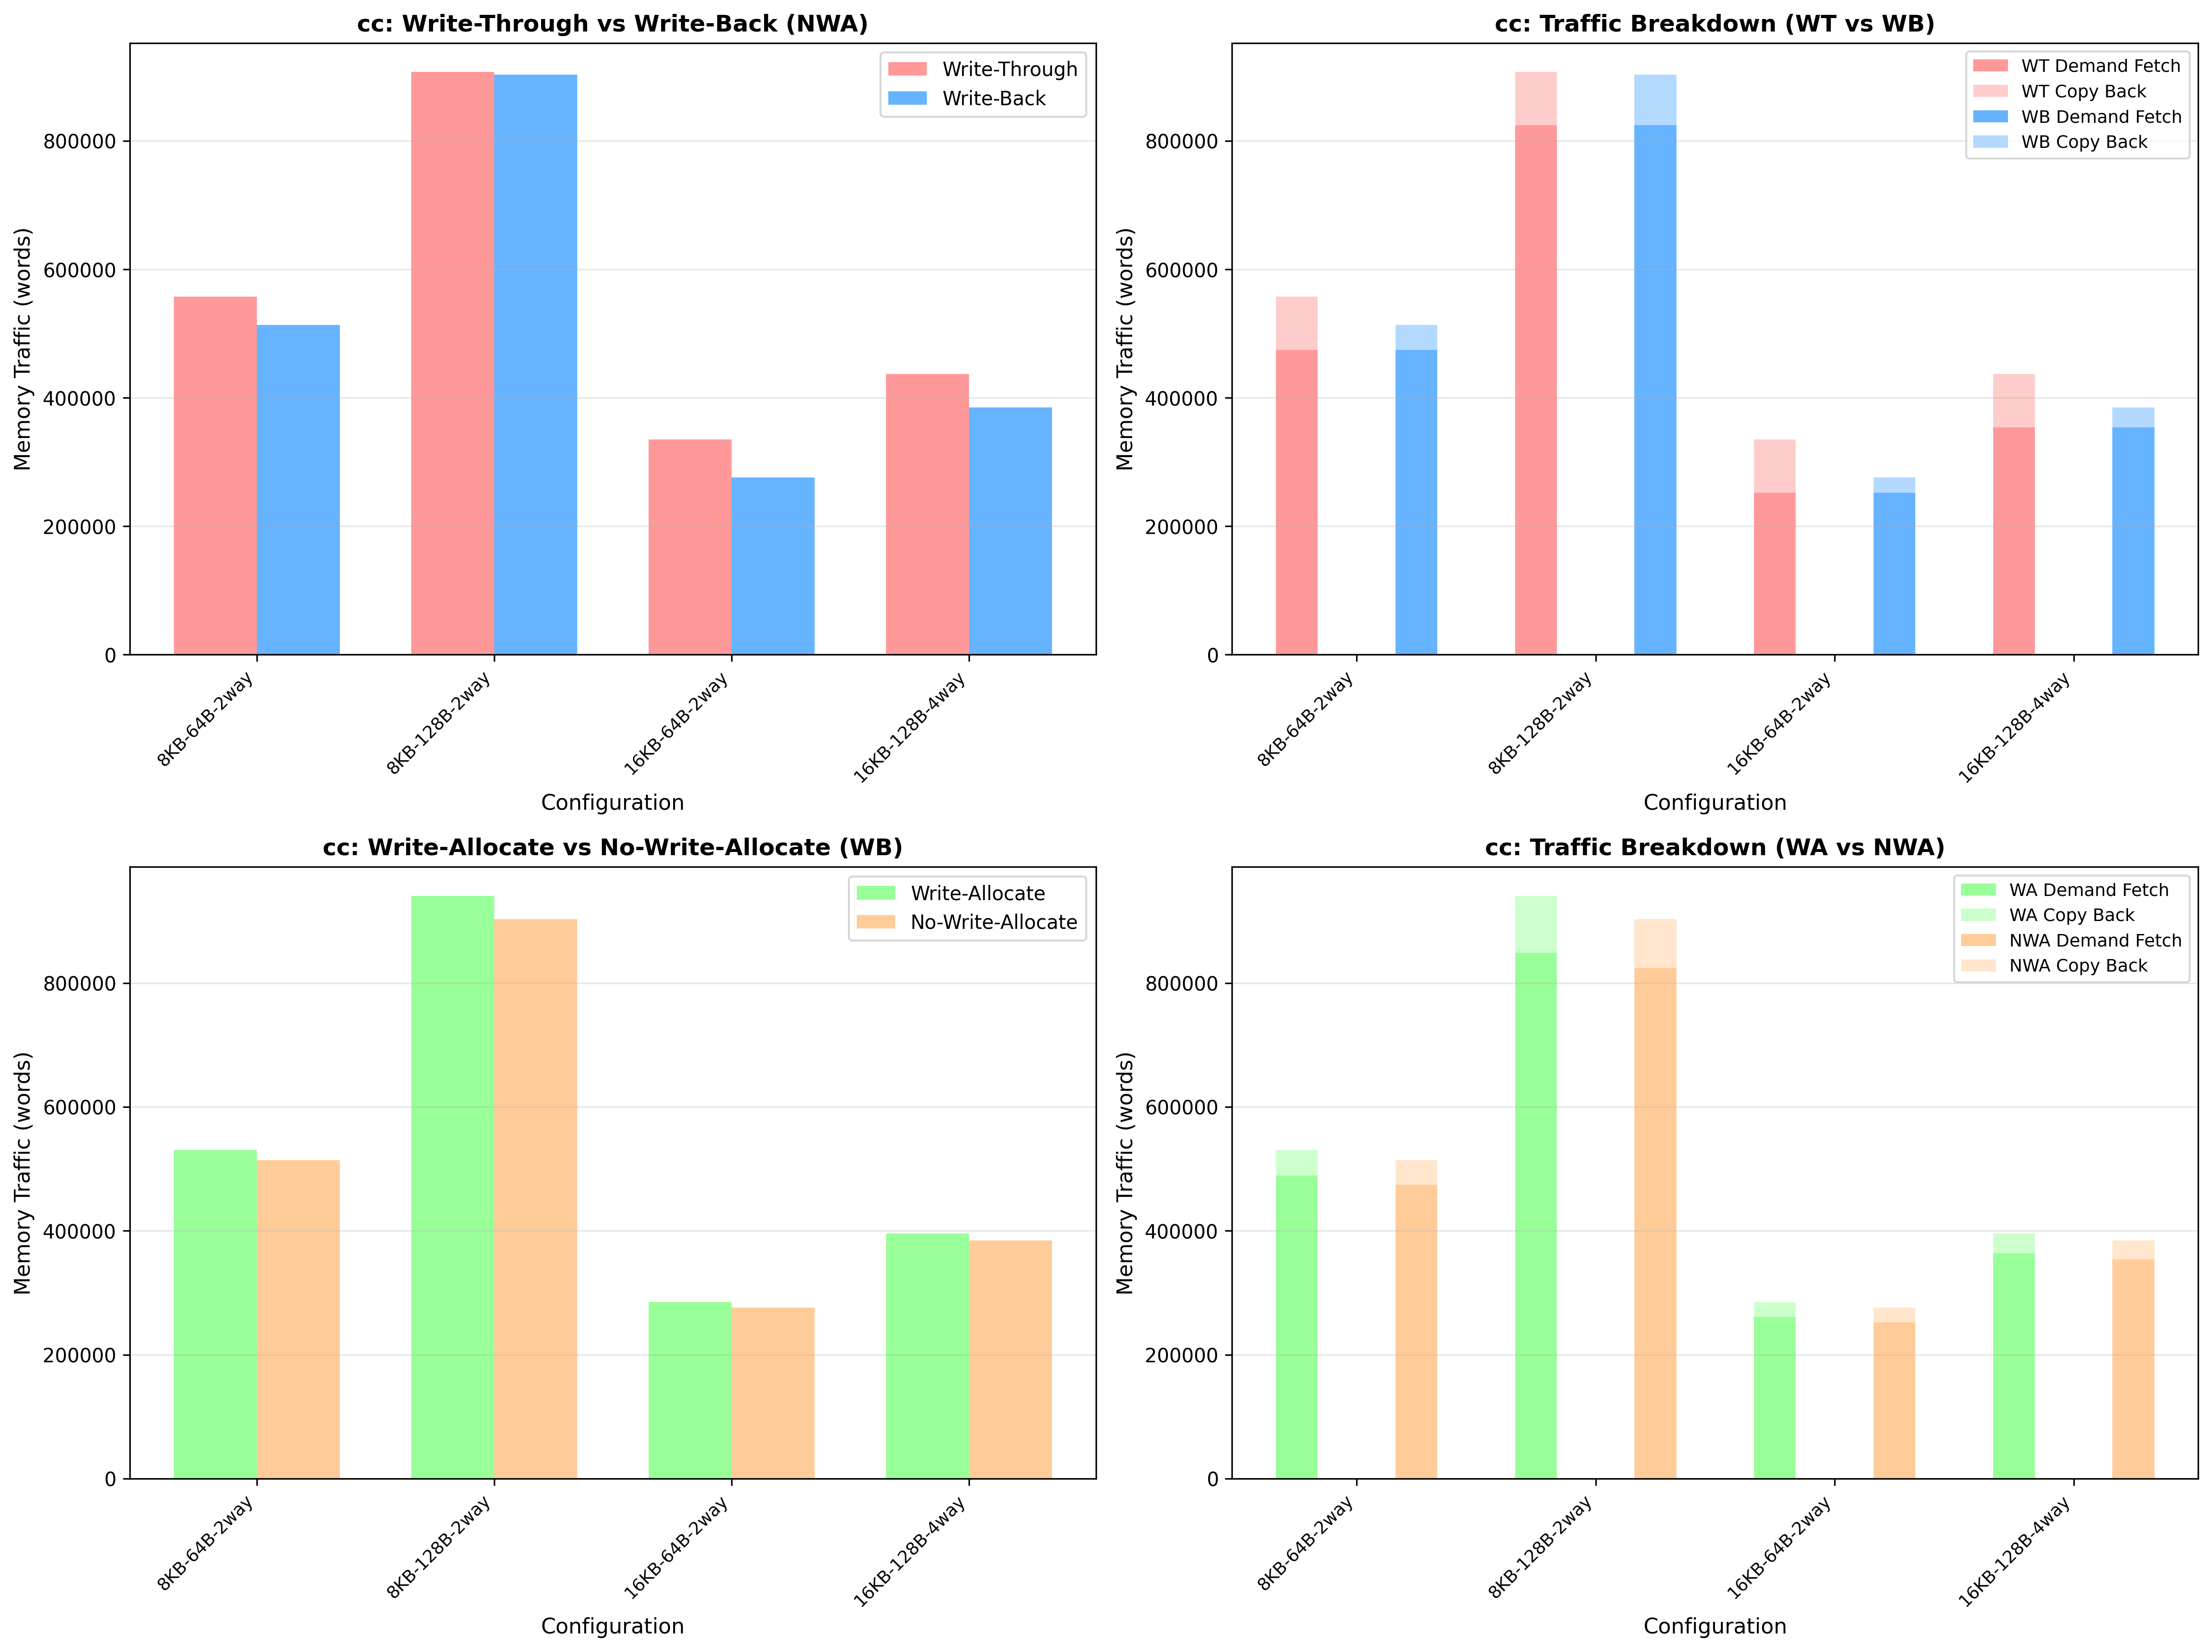
\includegraphics[width=0.9\textwidth]{memory_bandwidth_cc.png}
\caption{CC trace 内存带宽分析}
\end{figure}

\begin{figure}[H]
\centering
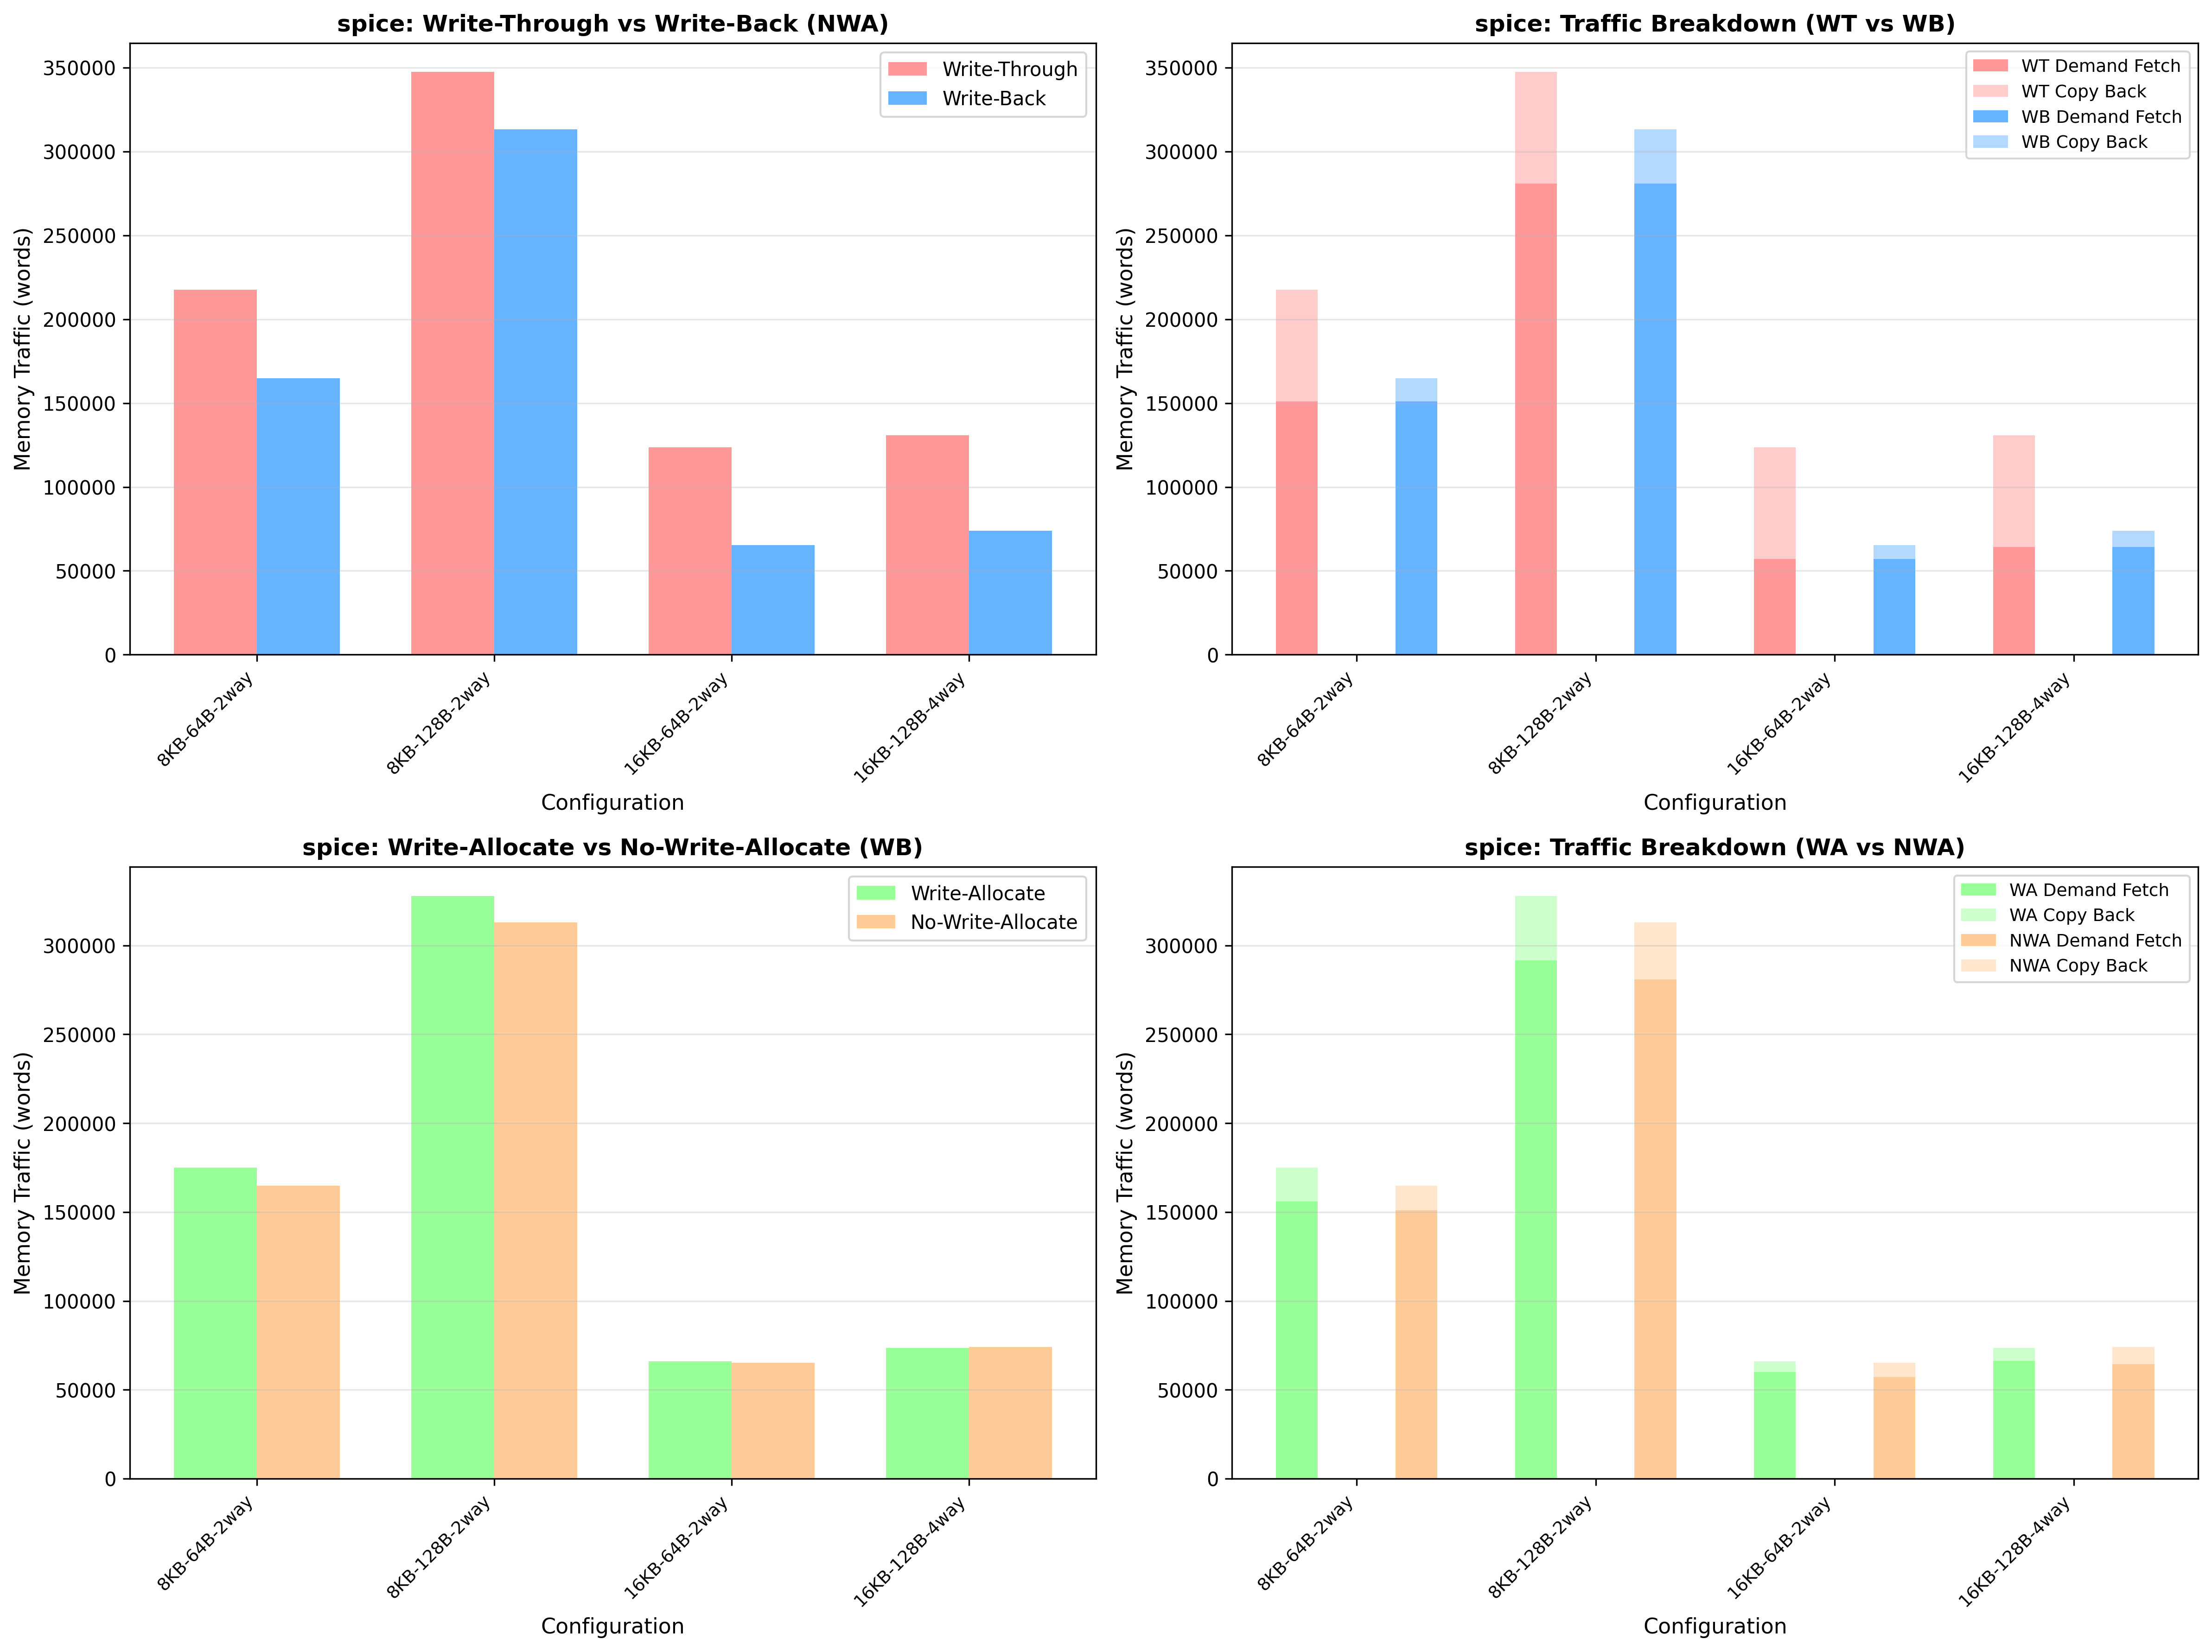
\includegraphics[width=0.9\textwidth]{memory_bandwidth_spice.png}
\caption{SPICE trace 内存带宽分析}
\end{figure}

\begin{figure}[H]
\centering
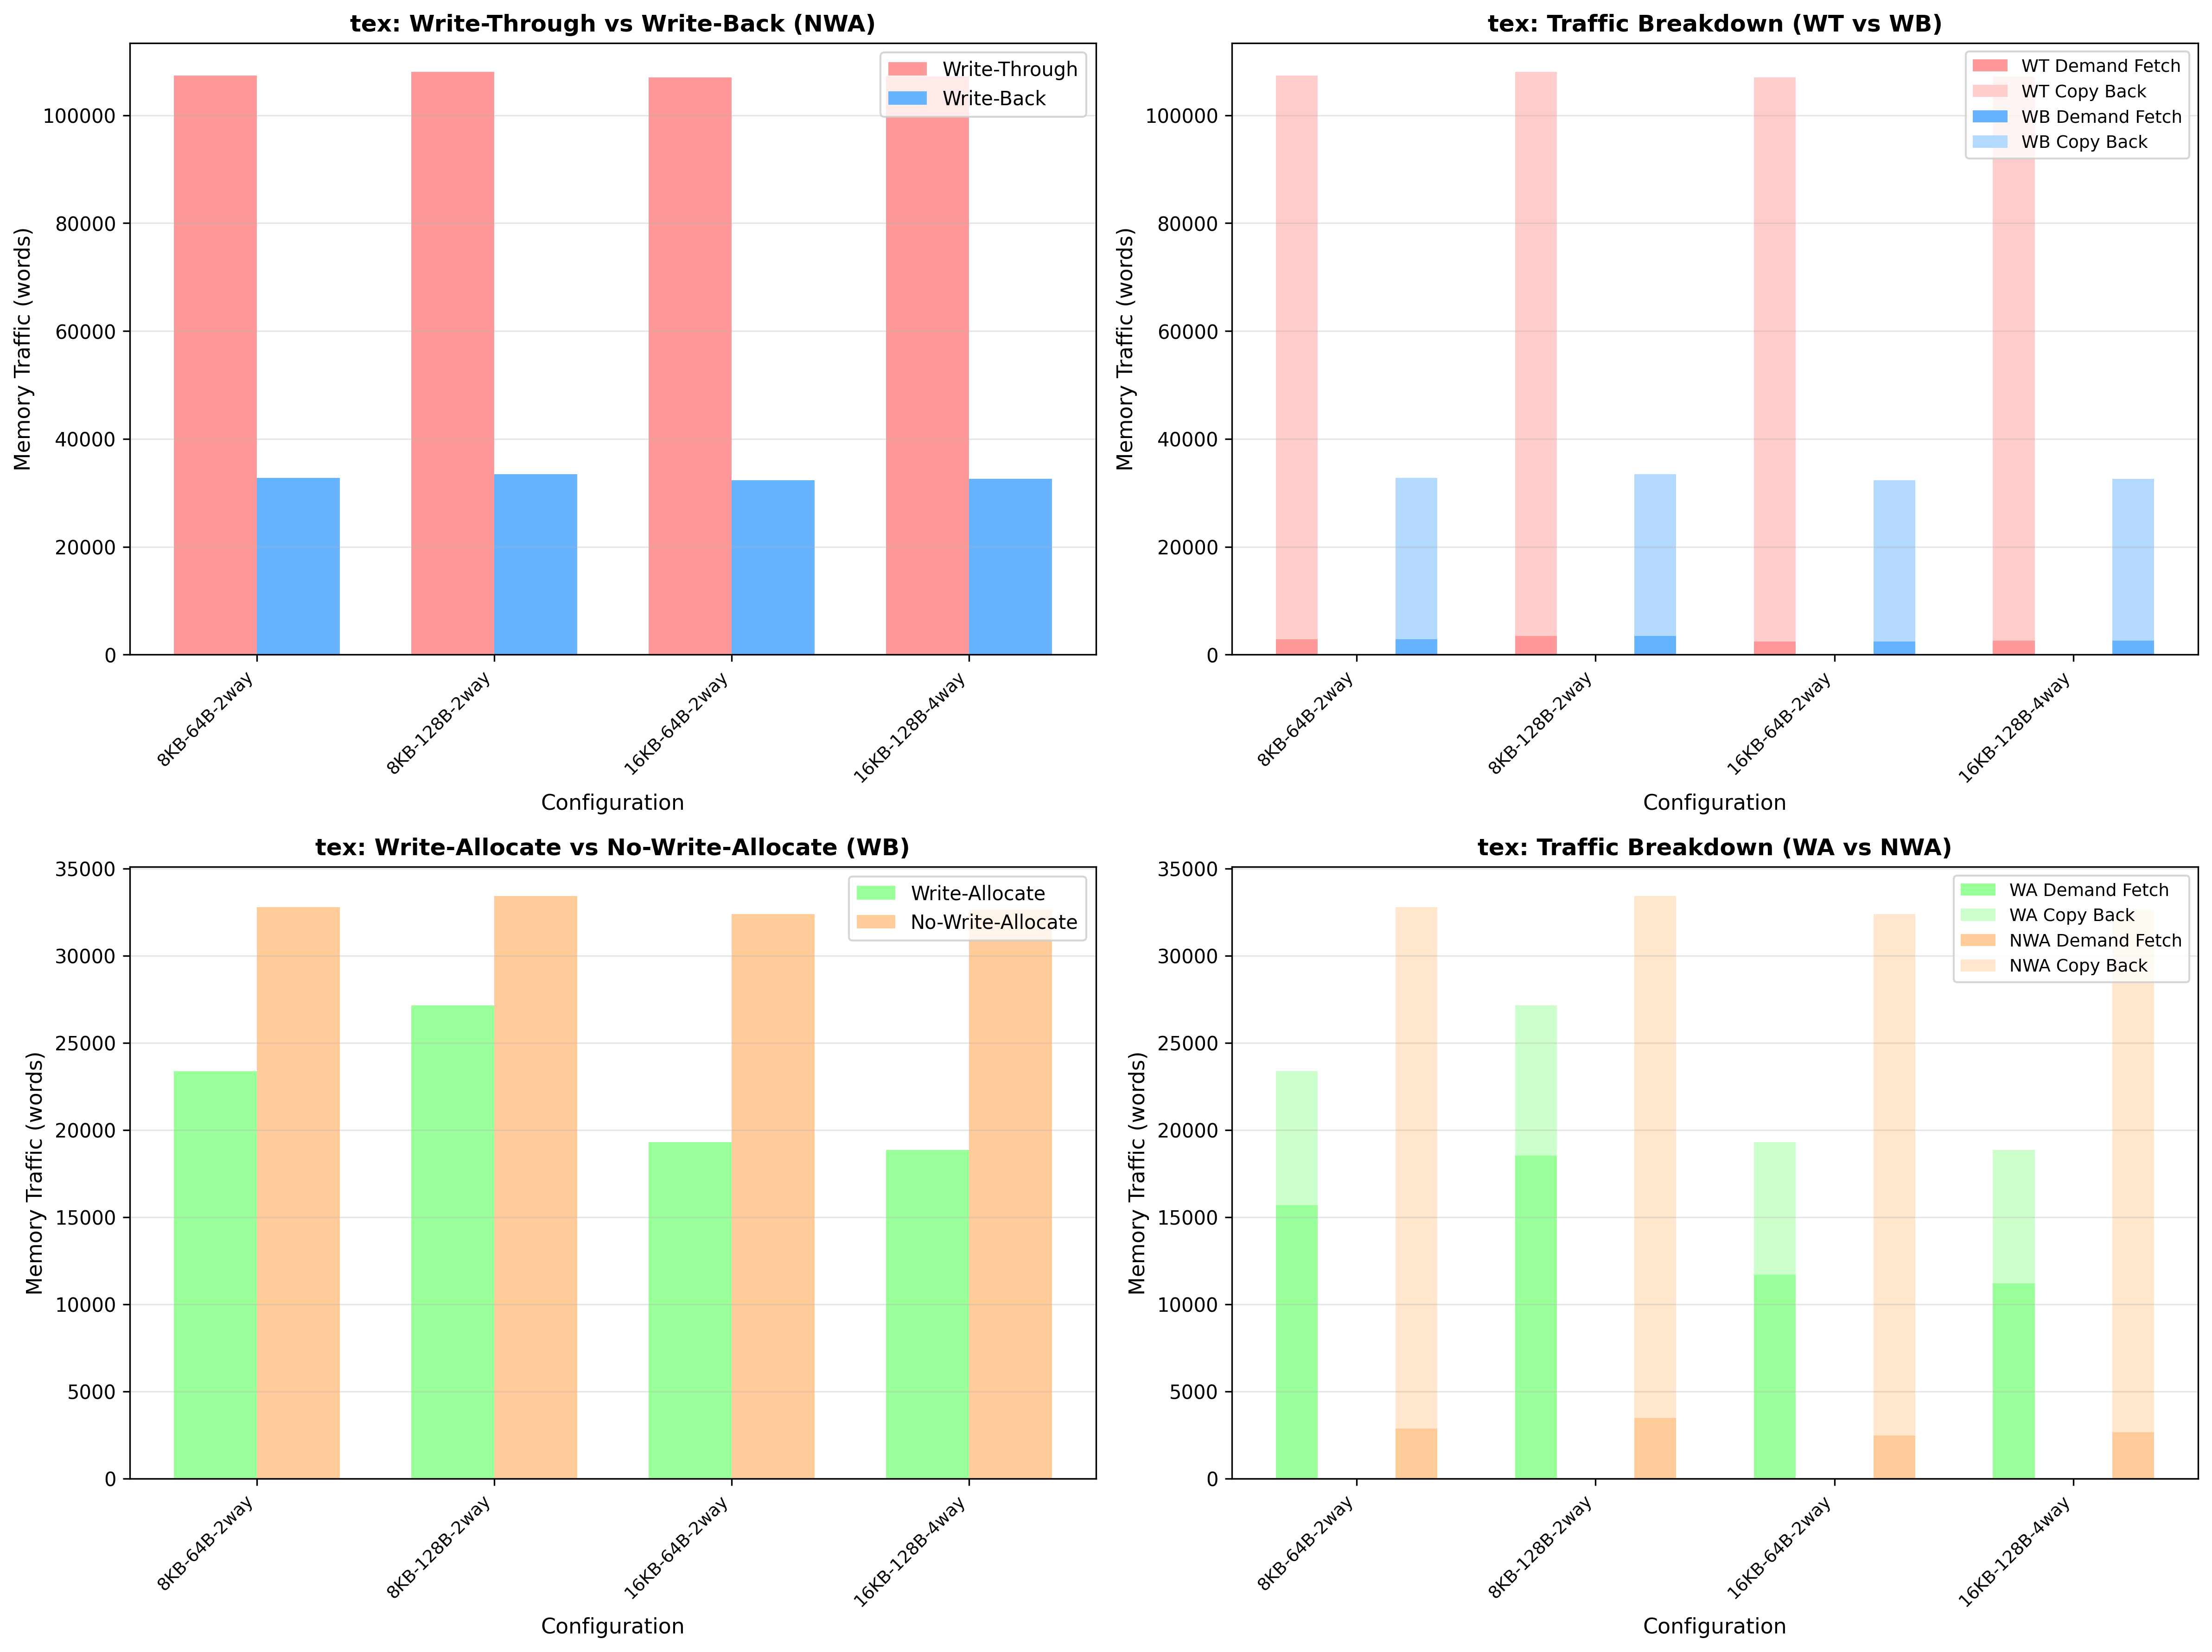
\includegraphics[width=0.9\textwidth]{memory_bandwidth_tex.png}
\caption{TEX trace 内存带宽分析}
\end{figure}

\subsubsection{结果分析}

\textbf{实验1：Write-Through vs Write-Back}

\begin{table}[H]
\centering
\caption{WB相对WT的内存流量减少}
\begin{tabular}{|l|c|}
\hline
\textbf{Trace} & \textbf{平均流量减少} \\
\hline
cc & 9.44\% \\
spice & 31.20\% \\
tex & 69.46\% \\
\hline
\end{tabular}
\end{table}

如表所示，Write-Back 缓存在所有测试中均产生\textbf{更少}的内存流量，流量减少幅度为 9.44\% 至 69.46\%。分析其原因如下：

\begin{table}[H]
\centering
\small
\caption{Write-Through 与 Write-Back 的行为对比}
\begin{tabular}{p{3.5cm}p{5.5cm}p{5.5cm}}
\toprule
\textbf{对比维度} & \textbf{Write-Through (WT)} & \textbf{Write-Back (WB)} \\
\midrule
写行为 & 每次写操作都立即写入内存（写命中写两次，写缺失写一次） & 写操作仅更新缓存并标记脏位，只在块驱逐时写回内存 \\
\midrule
时间局部性利用 & $N$ 次写 $\Rightarrow$ $N$ 次内存写 & $N$ 次写 $\Rightarrow$ 1 次内存写（驱逐时），\textbf{合并}了多次写操作 \\
\midrule
读流量 & demand fetches & demand fetches（与WT相同） \\
\midrule
写流量 & 所有写操作 & 仅脏块驱逐（$\ll$ 所有写操作） \\
\bottomrule
\end{tabular}
\end{table}

\textbf{结论反转的特殊场景：}

\begin{table}[H]
\centering
\small
\caption{WT 可能优于 WB 的特殊场景}
\begin{tabular}{p{3cm}p{5.5cm}p{6cm}}
\toprule
\textbf{场景} & \textbf{描述} & \textbf{原因分析} \\
\midrule
稀疏写入（Sparse Writes） & 程序具有极差的写局部性，且 Cache 块很大 & 假设块大小为 128 字节，CPU 仅修改其中 4 字节后该块就被替换：\newline \textbf{WT}：仅写入修改的 4 字节\newline \textbf{WB}：需写回整个 128 字节脏块\newline 写回传输了大量未修改的"废数据"，流量反而高于写直达 \\
\bottomrule
\end{tabular}
\end{table}

\textbf{实验2：Write-Allocate vs Write-No-Allocate}

\begin{table}[H]
\centering
\caption{WA vs NWA 流量差异}
\begin{tabular}{|l|c|}
\hline
\textbf{Trace} & \textbf{NWA相对WA的变化} \\
\hline
cc & +3.2\% (NWA更多) \\
spice & +2.2\% (NWA更多) \\
tex & -31.3\% (NWA更少) \\
\hline
\end{tabular}
\end{table}

如表所示，Write-Allocate 策略在 \textbf{cc} 和 \textbf{spice} 中产生更少的流量，而 Write-No-Allocate 在 \textbf{tex} 中表现更优。分析原因如下：

\begin{table}[H]
\centering
\small
\caption{Write-Allocate 与 Write-No-Allocate 的优劣分析}
\begin{tabular}{p{3.5cm}p{5.5cm}p{5.5cm}}
\toprule
\textbf{策略} & \textbf{优势场景} & \textbf{原因} \\
\midrule
Write-Allocate (WA) & 写入的数据很快被再次访问（cc、spice） & 写缺失时分配块，利用\textbf{后续读写的时间/空间局部性}，减少未来缺失，总流量更少 \\
\midrule
Write-No-Allocate (NWA) & "写后不读"的数据（tex 输出缓冲） & WA 浪费带宽取块且占用缓存空间造成污染，NWA 避免不必要的块分配 \\
\bottomrule
\end{tabular}
\end{table}

\textbf{应用场景建议：}

\begin{table}[H]
\centering
\small
\caption{WA vs NWA 的应用选择}
\begin{tabular}{p{4cm}p{11cm}}
\toprule
\textbf{工作负载类型} & \textbf{推荐策略} \\
\midrule
大多数通用应用 & Write-Allocate（利用时间/空间局部性） \\
\midrule
流式写入或输出密集型应用 & Write-No-Allocate 或非时态（Non-Temporal）写指令 \\
\bottomrule
\end{tabular}
\end{table}

\clearpage
\section{实验总结与实验心得}

\subsection{实验总结}

\begin{enumerate}
    \item \textbf{模拟器构建与验证}：成功实现了支持多种配置（总大小、块大小、关联度、写策略等）的迹驱动 Cache 模拟器，并通过了全部 22 组自动化测试用例的比对，验证了核心逻辑（如 LRU 替换、脏位管理）的正确性。
    
    \item \textbf{工作集特征分析}：通过改变 Cache 大小测定出 cc、spice 和 tex 三个 trace 的指令与数据工作集大小，观察到命中率曲线呈现"陡升（消除容量缺失）- 拐点 - 平台"的典型特征。
    
    \item \textbf{块大小影响分析}：证实了块大小存在最优值（Trade-off），过小无法利用空间局部性，过大则导致 Cache 污染和冲突增加；且发现指令 Cache 通常比数据 Cache 更受益于较大的块。
    
    \item \textbf{关联度影响分析}：验证了提高关联度可显著减少冲突缺失，但存在收益递减规律。实验揭示了指令流通常具有高度顺序性，对关联度要求较低（如 tex 在 1-way 即满命中），而数据流对关联度更敏感。
    
    \item \textbf{内存带宽与写策略}：数据表明 Write-Back 策略相比 Write-Through 能大幅减少（约 10\%-70\%）内存流量；Write-Allocate 策略通常更优，但在 tex 等流式输出场景下，Write-No-Allocate 表现更好。
\end{enumerate}

\subsection{实验心得}

通过本次实验，我不仅从代码层面掌握了 Cache 的查找、分配与回写机制，更通过对不同 Trace 的性能评估，深刻理解了"计算机体系结构设计在于权衡"这一核心思想。在探究块大小和关联度时，我直观地看到了空间局部性带来的收益以及 Cache 污染带来的负面影响，明白了参数配置并非单纯"越大越好"，而是取决于具体的访问模式。特别是 tex 在写分配策略上的反常表现（WNA 优于 WA），让我意识到针对流式写入等特定负载进行策略优化的重要性。这次实验将抽象的"局部性原理"和"冲突缺失"概念转化为可视化的数据曲线，极大地增强了我对存储层次结构设计复杂性的认知与工程实践能力。

\end{document}